\documentclass[a4paper,11pt]{article}
\usepackage[UKenglish]{babel}
\usepackage[utf8]{inputenc}
\usepackage[T1]{fontenc}
\usepackage{geometry}
\usepackage{amsmath}
\usepackage[dvipsnames]{xcolor}   %Colors
%-----------------------Pour figures
\usepackage{graphicx}
\usepackage{wrapfig}
\usepackage{hyperref}   %Pour liens hypertextes
%-----------------------Pour tableaux
\usepackage{caption}
\usepackage{array}
\usepackage{multirow}
\usepackage{multicol}
\usepackage{makecell}
\usepackage{adjustbox}
%------------------------------------
\usepackage{subcaption}
\usepackage{url}
\captionsetup{labelsep=period}
\usepackage[justification=centering]{caption}
\geometry{hmargin=2cm,vmargin=2cm}   %Marges
\usepackage{amssymb}
\usepackage{emptypage}
\usepackage{lineno}   %Pour numéroter les lignes
\usepackage[nogroupskip=true, acronym]{glossaries}   %Glossary
\usepackage[xindy]{imakeidx}
\usepackage{fancyhdr}
\pagestyle{fancy}
%\usepackage{csquotes}   %Pour les guillemets
%\MakeOuterQuote{"}   %Pour les guillemets
%-------------------------------------Pour biblio
\usepackage[sorting=none]{biblatex}   %Biblio
\addbibresource{Biblio.bib}   %Biblio file
\setlength\bibitemsep{1.8\itemsep}   %Space between bibliography entries

\usepackage[titletoc]{appendix}   %Pour annexes

\title{}
\author{Hind Taibi}
\date{}


\makeglossaries
\newacronym{ATLAS}{ATLAS}{A Toroidal LHC ApparatuS}
\newacronym{CERN}{CERN}{European Organization for Nuclear Research}
\newacronym{CMS}{CMS}{Compact Muon Solenoid}
\newacronym{FCC}{FCC}{Future Circular Collider}
\newacronym{HL-LHC}{HL-LHC}{High Luminosity-Large Hadron Collider}
\newacronym{IDEA}{IDEA}{Innovative Detector for Electron–positron Accelerators}
\newacronym{LAPP}{LAPP}{Laboratoire d'Annecy-le-Vieux de Physique des Particules}
\newacronym{LHC}{LHC}{Large Hadron Collider}
\newacronym{SM}{SM}{Standard Model}
\newacronym{VBF}{VBF}{Vector Boson Fusion}
\newacronym{PDF}{PDF}{Probability Density Function}
\newacronym{POI}{POI}{Parameter Of Interest}

%--------------------------------------
%	DOCUMENT
%--------------------------------------

\begin{document}
	
	%\linenumbers   %Pour numéroter les pages
	
	%--------------------------------------	
	%	TITLE PAGE
	%--------------------------------------
	
	\begin{titlepage}
		\begin{center}
			\begin{tabular}{c@{\hskip 4cm}c@{\hskip 1cm}}
				
\includegraphics[scale=0.45]{Paris-Saclay.png} &
				
\includegraphics[scale=0.45]{LAPP.png}
			\end{tabular}		 
		\end{center}
		
		\begin{center}
			
			\vspace*{.08\textheight}
			\textsc{\LARGE Université Paris-Saclay}\\[0.4cm]
			\large M1 Physique Fondamentale, MAG 2\\
			\vspace{40pt}
			
			\vfill
			
			\textbf{\LARGE Internship Report}\\
			\vspace{1cm}
			
			\large Laboratoire d'Annecy-le-Vieux de physique des particules\\
			9 chemin de Bellevue, 74941 ANNECY CEDEX\\
			
			\vspace{1cm}
			
					
			\rule{\textwidth}{1pt}
			\\ % Horizontal line
			\vspace{0.5cm}
			{\LARGE \bfseries Measurement of the \boldmath$ZH,H\rightarrow ZZ^*$ Cross Section in the Four Lepton Channel at FCC-ee} % Internship title
			\vspace{10pt}
			\rule{\textwidth}{1pt}\\ % Horizontal line
			\vspace{0.5cm}
		\end{center}
		
		\vspace{2cm}

		\begin{center}
			\textsc{\Large Hind Taibi}\\ (hind.taibi@universite-paris-saclay.fr)\\[1cm]
			Supervised by \textsc{\large Marco Delmastro} (marco.delmastro@lapp.in2p3.fr)\\[0.2cm]
			and \textsc{\large Olivier Arnaez} (olivier.arnaez@lapp.in2p3.fr)\\[0.2cm]
		\end{center}
		
		\vspace{3cm}
	
		\begin{center}
			Internship Carried Out From May 13th, 2024 to August 2nd, 2024\\
			2023-2024 Academic Year
		\end{center}
		
		\newpage %page de garde vide
		\thispagestyle{empty} %page de garde vide
	\end{titlepage}

	\pagenumbering{roman}
	
	%--------------------------------------
	%   EMPTY PAGE
	%--------------------------------------
	
	\newpage 
	\ % The empty page
	\newpage
	
	%--------------------------------------
	%	ABSTRACT PAGE
	%--------------------------------------

	\noindent
	{\Large\textbf{Abstract}}\\\\
	The Higgs boson, predicted by P. Higgs, R. Brout and F. Englert in 1964 and discovered in 2012 at the LHC by ATLAS and CMS collaborations, is the latest discovered component of the Standard Model of particle physics. Since its discovery, studying its properties and measuring them with high precision has been one of the objectives of the particle physics community. The FCC project is at the centre of this enterprise. Among the properties that are planned to be measured at the FCC-ee, stands the Higgs width that can be measured at an electron-positron collider with the minimal theoretical assumptions. This can be achieved by simultaneously measuring the inclusive $e^+e^-\rightarrow ZH$ cross section, and the $e^+e^-\rightarrow ZH,H(ZZ^*)$ cross section.\\\\
	This internship report is about the measurement of the $e^+e^-\rightarrow ZH,H(ZZ^*)$ cross section at FCC-ee based on FCC-ee simulations. The main purpose of the internship was to analyse simulated data of signal and background for specific decay channels where we have four leptons in the final state to see how much the background would taint the measurement and estimate the channels sensitivity.\\\\
    %\textbf{Keywords}: Higgs boson, FCC-ee, Higgs width, Higgs Strahlung.
    \\\\\\\\\\\\
	
	\noindent
	{\Large\textbf{Résumé}}\\\\
	Le boson de Higgs, prédit par P. Higgs, R. Brout et F. Englert en 1964 et découvert en 2012 au LHC par les collaborations ATLAS et CMS, est la dernière composante du Modèle standard de la physique des particules à être découverte. Depuis sa découverte, l'étude de ses propriétés et leur mesure avec une grande précision fait partie des objectifs de la communauté de la physique des particules. Le projet FCC se trouve au centre de cette quête. Parmi les propriétés que l'on compte mesurer au FCC-ee, il y a la largeur du boson de Higgs qui peut être mesurée dans un collisionneur électron-positron avec le minimum d'hypothèses théoriques. Pour ce faire, on mesure simultanément la section efficace du processus $e^+e^-\rightarrow ZH$, et la section efficace du processus $e^+e^-\rightarrow ZH,H(ZZ^*)$.\\\\
	Ce rapport de stage porte sur la mesure de la section efficace de $e^+e^-\rightarrow ZH,H(ZZ^*)$ au FCC-ee à partir de simulations FCC-ee. L'objectif principal de mon stage était d'analyser des données simulées de signal et de bruits de fond pour des canaux où l'on a quatre leptons dans l'état final pour voir à quel point le fond entacherait la mesure de la largeur et estimer la sensibilité des canaux.
    %\textbf{Mots-clés} : boson de Higgs, FCC-ee, largeur du boson de Higgs, Higgs Strahlung.
	
	%--------------------------------------
	%	AKNOWLEDGEMENTS PAGE
	%--------------------------------------   
	
	\newpage
	\noindent
	{\Large\textbf{Aknowledgements}}\\\\
    My internship at LAPP was one of the most pleasant and stimulating experiences I have had in my academic journey. I was excited to go there every day thanks to its warm and friendly environment. Many thanks to the whole ATLAS team of LAPP for that.\\\\
    Mes remerciements les plus sincères à mes deux encadrants de stage, Marco Delmastro et Olivier Arnaez, pour m'avoir si bien accompagnée pendant mon stage et pour m'avoir emmenée au CERN ! J'ai énormément appris grâce à eux et discuter avec eux a toujours été un réel plaisir. Je n'en aurai jamais assez d'écouter des anecdotes sur la découverte du boson de Higgs.\\\\
    Merci à Ines Combes dont le précédent travail sur l'analyse FCC-ee m'a servi de point de départ pour mon stage et à Nicolas Morange de l'IJCLab pour avoir répondu à nos interrogations.
    %Enfin je remercie mes parents qui ont dû, je pense, m'écouter parler de mon stage tous les jours pendant trois mois, et qui m'ont fait grandir dans un environnement portant un grand intérêt pour la physique. C'est grpace à eux que je me suis dirigiée vers ce milieu et que je m'y épanouis.
    
	%--------------------------------------
	%	CONTENTS PAGE
	%--------------------------------------	
	
	\newpage
	\pagenumbering{arabic}
	\tableofcontents
	\newpage

	\printindex

    %--------------------------------------
	%	GLOSSARY AND LISTS PAGE
	%--------------------------------------
	
	\addcontentsline{toc}{section}{\protect\numberline{}Acronyms}
	\printglossary[type=\acronymtype]

    \newpage
	\addcontentsline{toc}{section}{\protect\numberline{}List of Figures}
    \listoffigures
	
	\addcontentsline{toc}{section}{\protect\numberline{}List of Tables}
    \listoftables
	
	%--------------------------------------
	%	LET THE REPORT BEGIN
	%--------------------------------------
		
	\newpage
	\section{Introduction}
	The Standard Model of particle physics is an elegant mathematical framework that was built over the 20th century to describe the nature of particles, their dynamics and three out of the four fundamental interactions: the electromagnetic interaction which is responsible for the atomic structure, the weak interaction which is responsible for radioactive decays and the strong interaction which confines quarks into hadrons and binds neutrons and protons into nuclei. The gravitational interaction is yet to be explained by the Standard Model. It took a long time to build the Standard Model. Indeed, its first particle, the electron, was discovered in 1899 by J. J. Thomson, and its last one, the Higgs boson, was only discovered in 2012 by \acrshort{ATLAS} \cite{atlas2012observation} and \acrshort{CMS} \cite{cms2012observation} collaborations at the \acrshort{LHC}. It is so far the most accurate and dominant theory explaining the behaviour of particles and their interactions and it has been well supported by experimental observations.\\\\
	The Higgs Boson was predicted by P. Higgs \cite{higgs1964broken}; R. Brout and F. Englert \cite{englert1964broken}; G. Guralnik, C. Hagen and T. Kibble \cite{guralnik1964global} in 1964 to explain the origin of the mass of gauge bosons without breaking the gauge symmetry of the Standard Model. Later, a Yukawa interaction with the Higgs field was added to also generate mass for fermions. The discovery of the Higgs boson in 2012 makes it the particle with the longest time interval between its prediction and its discovery. Following the discovery of this last piece of the Standard Model, the goal has been moved to studying its properties, such as its couplings to other particles and its width, 
	and measuring them with high precision. Finding signs of physics beyond the Standard Model is one of the main challenges of modern physics and the Higgs boson may be a gateway to this new physics. The construction of a new accelerator larger than the LHC where one could precisely determine the properties of the Higgs boson would be a big step in the exploration of high energy physics and in this regard, the FCC project, a 91 km long circular collider, was proposed.\\\\
	The \acrshort{FCC} will feature as a first stage an electron-positron collider (FCC-ee) before hosting a hadron collider (FCC-hh) during its second stage. In terms of energy, electron-positron colliders can hardly compete with hadron colliders because of the synchrotron radiation. However, electron-positron colliders present a better signal over background ratio. Another advantage of having an electron-positron collider is knowing completely and precisely the kinematic properties of the initial state since the electron and the positron are elementary particles.\\\\
	The Higgs boson width stands within one of the properties covered by the FCC-ee physics program. It is predicted by the Standard Model to be around 4 MeV, a value that cannot be directly measured at the LHC without making assumptions about the model while the FCC-ee will allow us to measure the Higgs width model-independently with minimal theoretical assumptions.\\\\
	The goal of my internship at \acrshort{LAPP} within the ATLAS/FCC team was to study the measurement of the $e^+e^-\rightarrow ZH,H(ZZ^*)$ cross section in the four lepton channel, a crucial ingredient to the Higgs width determination. In the first section of this report, I introduce the FCC-ee project and some elements of the Higgs physics in this future collider. The second section is about the different decay channels that have been considered as well as the backgrounds. The analysis and the results will then be discussed in a final section.
	
	\newpage
	\section{The Higgs boson at FCC-ee}
	%The aim of this section is to give an overview of the FCC project and its physics program, especially during the FCC-ee stage which is the stage  in which we are interested in this study.
 
	\subsection{The FCC Project}
    \begin{wrapfigure}{r}{0.4\textwidth}
        \centering
        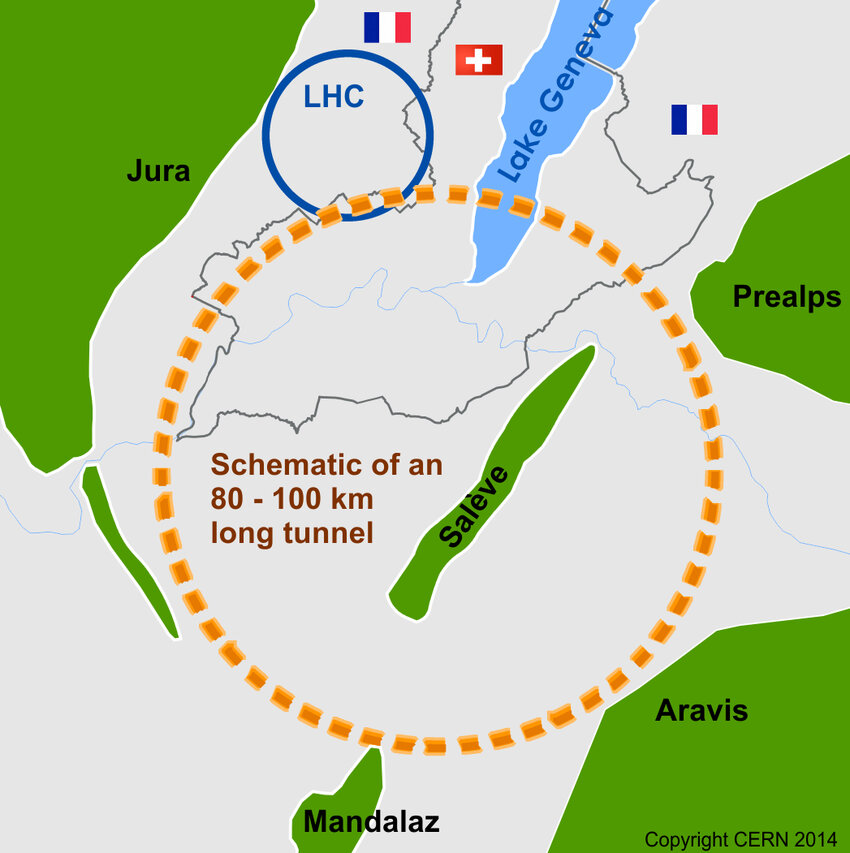
\includegraphics[width=0.36\textwidth]{FCCee.jpg}
        \caption{Scheme of a possible location for the FCC.}
        \label{FCCee}
    \end{wrapfigure}
    The FCC is a future particle accelerator with a planned circumference of about 91 km \cite{zimmermann2023jacow} that would follow on from the \acrshort{HL-LHC}. It would be built next to the LHC (see Figure~\ref{FCCee}) and host up to four experiments. The first stage of the FCC, the FCC-ee, consists in a high luminosity electron-positron collider serving as Higgs and electroweak factory which would first operate at a centre of mass energy of $\sqrt{s}=240$ GeV and then at $\sqrt{s}=365$ GeV. With an integrated luminosity of $L=5$ ab$^{-1}$ corresponding to the production of $10^6$ Higgs bosons approximately, the FCC-ee is designed to carry out precision measurements of the Higgs properties. The FCC-hh, which will mainly be a proton-proton collider, would succeed to the FCC-ee as the FCC's second stage and share the same tunnel and technical infrastructure. The FCC-hh is expected to reach at least $\sqrt{s}=100$ TeV of proton-proton collisions with the objective of exploring high energy physics even further. In comparison, the LHC is currently operating at $\sqrt{s}=13.6$~TeV.\\\\
    This internship falls within the ongoing feasibility study of the FCC-ee which should be concluded in 2025 and provide the necessary input for \acrshort{CERN} Member States and international partners to take a decision regarding this project in the course of 2027-2028.
 
	\subsection{Higgs Production at FCC-ee} \label{HiggsProductionFCCee}
    At electron-positron colliders, such as FCC-ee, the Higgs boson is produced through two main processes: Higgs-Strahlung ($ZH$) and vector boson fusion (\acrshort{VBF}). Figure \ref{HiggsFD} illustrates their Feynman diagrams at leading order.\\
    \begin{figure}[ht]
        \begin{minipage}[c]{0.68\linewidth}
            \centering
            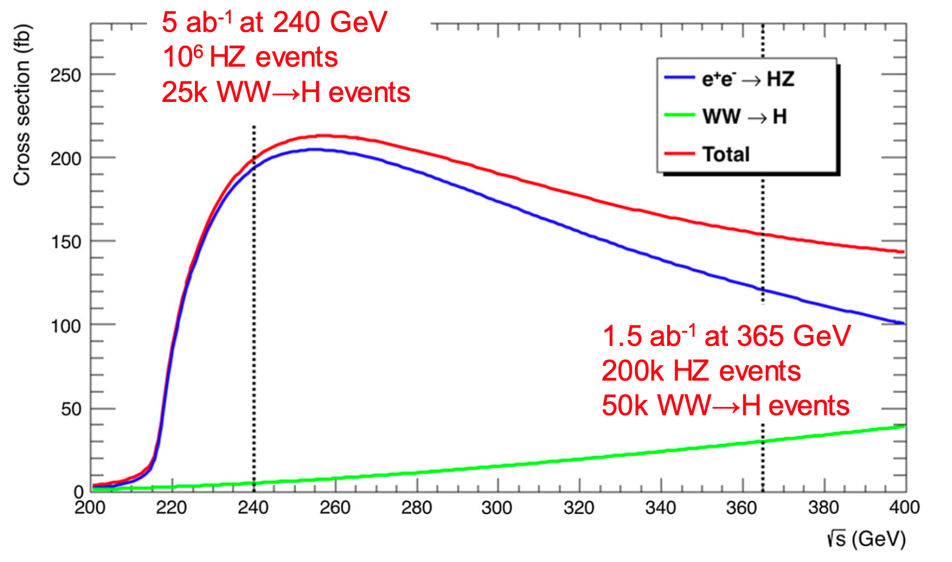
\includegraphics[scale=0.55]{HiggsCS.png}
            \caption{VBF and $ZH$ cross sections as functions\\of the centre of mass energy at electron-positron collider.}
            \label{HiggsCS}
        \end{minipage}      
        \begin{minipage}[c]{0.32\linewidth}
            \centering
            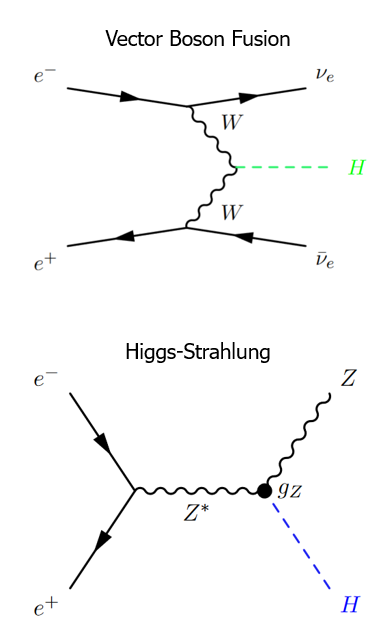
\includegraphics[scale=0.5]{HiggsFD.png}
            \caption{VBF and $ZH$ Feynman diagrams\\at leading order.}
            \label{HiggsFD}
        \end{minipage}
    \end{figure}

    \newpage
    \noindent
    The number of events of a a given process is given by:
    \begin{equation}
        N_{\mbox{events}}=L\times\sigma
    \end{equation}
    where $L$ is the integrated luminosity and $\sigma$ is the cross section of the process.\\\\
    The Higgs-Strahlung process, which is the leading Higgs production process, is particularly interesting because the production of the Higgs boson is associated with the production of a $Z$ boson. Therefore, the Higgs signal can be tagged through the associated $Z$ decay, especially if this $Z$ boson decays into a pair of leptons (an electron-positron pair or a muon-antimuon pair) which can be clearly tagged and are precisely measured by particle detectors. At FCC-ee, the $ZH$ mechanism will be drawn on at $\sqrt{s}=240$ GeV where its cross section is not maximal (see Figure \ref{HiggsCS}) but where its rate, compared to VBF, is.\\
    \begin{wrapfigure}{r}{0.45\textwidth}
        \vspace{-20pt}
        \centering
        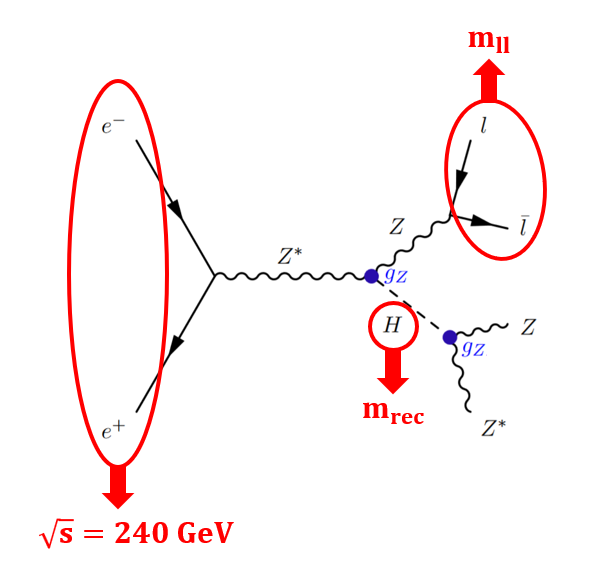
\includegraphics[scale=0.5]{RecoilFD.png}
        \caption{$ZH,H(ZZ^*)Z(ll)$ Feynman diagram.}
        \label{RecoilFD}
    \end{wrapfigure}
    Through Higgs-Strahlung, one can measure the $ZH$ inclusive cross section, called $\sigma_{ZH}=\sigma(ee\rightarrow ZH)$, model independently without making any assumption on the Higgs decay and its branching ratios. To do so, the recoil method is used. This method consists in calculating the recoil mass, $m_{\mbox{rec}}$, of the dilepton into which decays the $Z$ boson in $ZH$ (see Figure \ref{RecoilFD}). The recoil mass is the invariant mass of the dilepton four-vector from which is subtracted the initial state four-vector. It should be around 125 GeV (the Higgs mass) and is given by:
    \begin{equation}
        m^2_{\mbox{rec}}=(\sqrt{s}-E_{ll})^2-p^2_{ll}
    \end{equation}
    where $E_{ll}$ is the energy of the dilepton and $p_{ll}$ its momentum.\\\\
    The FCC-ee being an electron-positron collider, the initial state four-vector is completely known and thus the recoil mass can be experimentally measured without any theoretical assumptions. The recoil mass spectrum gives us access to the Higgs mass and the inclusive cross section $\sigma_{ZH}$ \cite{ruan2016elsevier} through the proportional relationship:
    \begin{equation}
        \sigma_{ZH}\propto g^2_Z
    \end{equation}
    where $g_Z$ is the coupling between the Higgs boson and the $Z$ boson.\\\\
    This report focuses on the $ee\rightarrow ZH,H(ZZ^*)$ process which is a specific case of $ZH$. By considering the specific decay where the Higgs boson decays into two $Z$ bosons, one being on-shell ($Z$) and the other being off-shell ($Z^*$), one can access the total Higgs width through the relation:
    \begin{equation}
        \Gamma_H=\frac{\sigma_{ZH}}{\sigma_{ZH,H(ZZ^*)}}\Gamma_{H\rightarrow ZZ^*}
    \end{equation}
    where $\sigma_{ZH,H(ZZ^*)}=\sigma(ee\rightarrow ZH,H(ZZ^*))$ is the cross section of $ZH,H(ZZ^*)$, and $\Gamma_{H\rightarrow ZZ^*}$ is the Higgs width associated to the $H\rightarrow ZZ^*$ decay.\\\\
    In a nutshell, the Higgs production at FCC-ee would allow us to experimentally measure $\sigma_{ZH}$ through the recoil method and then deduce the coupling $g_Z$ to compare it with the \acrshort{SM} predictions, reducing the theoretical input to the sole $\Gamma_{H\rightarrow ZZ^*}$ calculations whose theoretical uncertainty is lower than 1 \% \cite{lhc2011standard}. A deviation from the SM predictions would be a sign of physics beyond the Standard Model. We would also be able to measure the Higgs width ($\Gamma_H$) using $\sigma_{ZH}$ and $\sigma_{ZH,H(ZZ^*)}$ cross sections.
    
	\subsection{IDEA: Detector Concept at FCC-ee}
    \acrshort{IDEA} is one of the projects in development for the FCC and the detector concept used for the data simulations that I have been using during my internship. It is conceptually similar to ATLAS and CMS; it is made in a concentric design starting, from inside to outside, with an internal tracking system surrounded by electromagnetic and hadronic calorimeters and ending with a muon detector \cite{idea2022}.
    \begin{wrapfigure}{r}{0.53\textwidth}
        \centering
        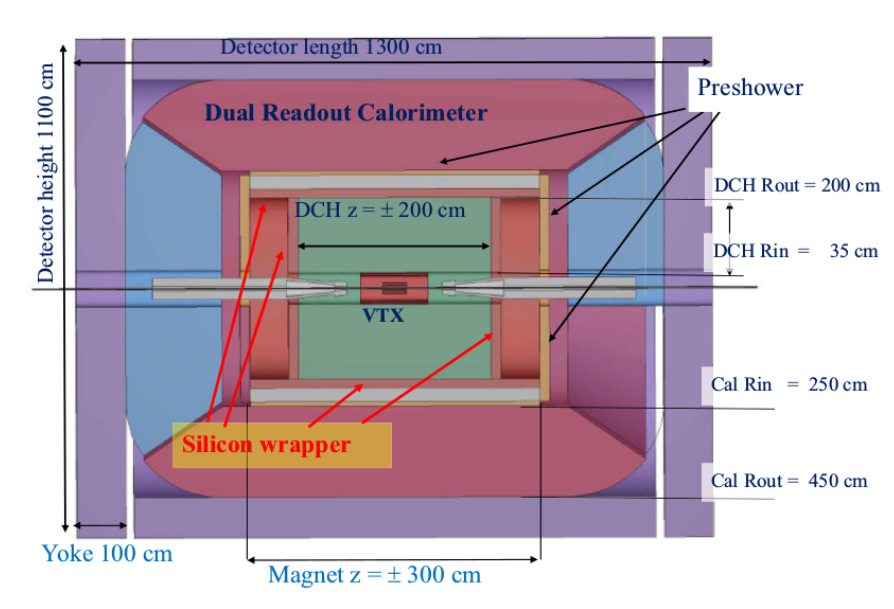
\includegraphics[scale=0.28]{IDEA.png}
        \caption{Sketch of the IDEA detector layout.}
        \label{IDEA}
        \vspace{-30pt}
    \end{wrapfigure}
    As shown in Figure \ref{IDEA}, it consists of:
    \begin{itemize}
        \itemsep0em 
        \item A silicon pixel vertex detector;
        \item A large-volume extremely-light drift wire chamber;
        \item A layer of silicon micro-strip detectors;
        \item A thin low-mass superconducting solenoid coil (optimized at 2 T) to maximize luminosity;
        \item A preshower detector;
        \item A dual read-out calorimeter;
        \item Muon chambers inside the magnet return yoke.
    \end{itemize}
    The $Oz$ axis is defined as being the beam axis. Two angles are defined from $Oz$: $\theta\in[0,\pi]$ and $\varphi\in[-\pi,\pi]$. $\theta$ being the angle between the particle and the beam axis and $\varphi$ being the angle of the particle on the transverse plane.\\\\
    For the data analysis, which will be detailed in section \ref{EventsReconstruction}, one would like to extract many kinematic variables regarding the leptons (electrons, muons and their antiparticles), the jets and the neutrinos. The electrons and muons (and their antiparticles), alongside the photons and the quarks, which are used to reconstruct jets, are directly detected and their kinematic properties are directly measured. On the other hand, neutrinos, which only interact through weak interaction, cannot be detected in this type of detector. They are therefore invisible and so is their four-vector, this is why they are reconstructed from the missing kinematic information. Indeed, conservation laws impose the conservation of energy and momentum in the centre of mass frame. The undetected kinematic properties of the neutrinos appear in a form of missing variables.

	\section{Events Reconstruction} \label{EventsReconstruction}
    This section is dedicated to the detail of the data analysis explaining how the events have been reconstructed from the raw simulated data and introducing the different sources of background.\\\\
    \underline{Note}: in the following sections, leptons refer to electrons, muons and their antiparticles. We do not consider the tau lepton because it is not directly detected as such. Indeed, due to its short lifetime ($2.8\;10^{-13}$ s), it decays inside the beam pipe. At ATLAS for instance, it is reconstructed from jets \cite{Friedrich_2012}. Neutrinos are explicitly cited as neutrinos and quarks are usually referred to as jets. Also, I confuse particles and their antiparticles for practicality; "electrons" would refer to both electrons and positrons for example. Thus, a "leptonic $Z$ boson" implies that the $Z$ boson talked about has decayed into either one electron and one positron or one muon and one antimuon.
    
	\subsection[$ZH,H(ZZ^*)$ Four Lepton Final States]{\boldmath$ZH,H(ZZ^*)$ Four Lepton Final States} \label{DecayChannels}
    As emphasized in section \ref{HiggsProductionFCCee}, $ZH,H(ZZ^*)$ is what we consider being the signal in this study. We have three $Z$ bosons, two on-shell $Z$ bosons and one off-shell $Z$ boson, and each one of them can decay into either two leptons, two neutrinos or two quarks following the fractions listed in Table \ref{ZDecaysFractions}. We choose to call $Z_1$ the $Z$ boson accompanying the Higgs boson and for the $Z$ bosons into which this latter decays, the on-shell $Z$ is called $Z_2$ and the off-shell $Z$ is called $Z_3$ (see Figure \ref{ZDecaysFD}).\\\\
    In addition to considering the $ZH,H(ZZ^*)$ decay, we are interested in the specific final state in which there are four leptons, meaning that two out of the three $Z$ bosons have decayed into a pair of leptons. We are thus considering the six cases listed below.
    \begin{equation}
        \mbox{2 on-shell leptonic $Z$ bosons:} \left\{
        \begin{array}{ll}
            Z_1(\textcolor{red}{ll})Z_2(\textcolor{red}{ll})Z_3(\textcolor{NavyBlue}{jj}) \\
            Z_1(\textcolor{red}{ll})Z_2(\textcolor{red}{ll})Z_3(\textcolor{Green}{\nu\nu}) 
        \end{array}
        \right.
        \label{2OnShell}
    \end{equation}
    \begin{equation}
        \mbox{1 on-shell and 1 off-shell leptonic $Z$ bosons:} \left\{
        \begin{array}{ll}
            Z_1(\textcolor{red}{ll})Z_2(\textcolor{NavyBlue}{jj})Z_3(\textcolor{red}{ll}) \\
            Z_1(\textcolor{NavyBlue}{jj})Z_2(\textcolor{red}{ll})Z_3(\textcolor{red}{ll}) \\
            Z_1(\textcolor{red}{ll})Z_2(\textcolor{Green}{\nu\nu})Z_3(\textcolor{red}{ll}) \\
            Z_1(\textcolor{Green}{\nu\nu})Z_2(\textcolor{red}{ll})Z_3(\textcolor{red}{ll})
        \end{array}
        \right.
        \label{1OnShell1OffShell}
    \end{equation}
    Mixed final states with different combinations of $ll\;jj\;\nu\nu$ and final states with four jets have already been studied by Ines Combes \cite{InesCombes2023}.
    
    \begin{table}[ht]
    \begin{minipage}[h]{0.6\textwidth}
        \centering
        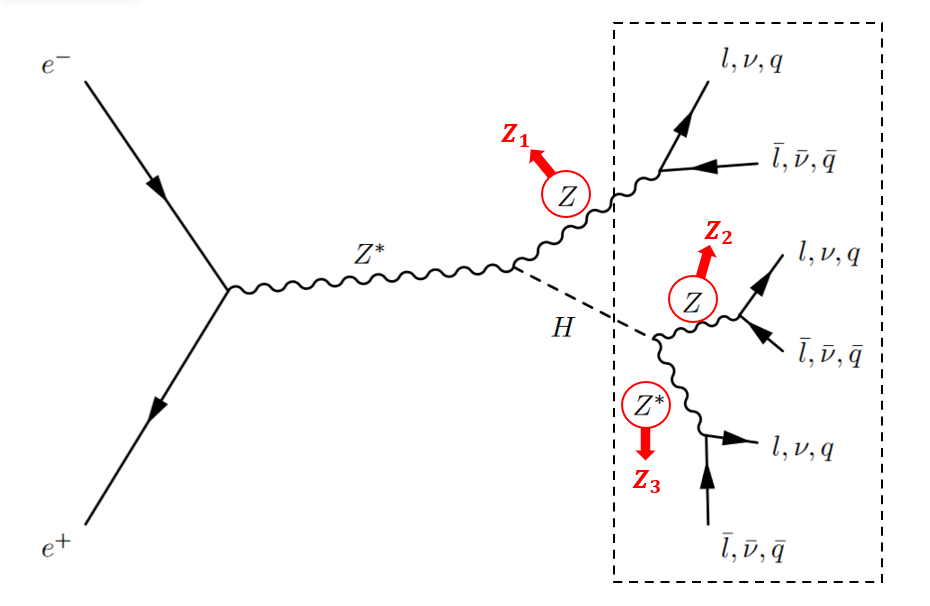
\includegraphics[scale=0.5]{ZDecaysFD.png}
        \captionof{figure}{$ZH,H(ZZ^*)$ Feynman diagram with possible decays of the $Z$ bosons.}
        \label{ZDecaysFD}
    \end{minipage}
    \begin{minipage}[h]{0.4\textwidth}
        \centering
        \begin{tabular}{|c|c|}\hline
            Decay & Fraction \\ 
            \hline
            \makecell{$l\bar{l}$ \\ ($e^-e^+$, $\mu^-\mu^+$, $\tau^-\tau^+$)} & $\sim 10$ \% \\
            \hline
            \makecell{$\nu\bar{\nu}$ \\ ($\nu_e\bar{\nu}_e$, $\nu_\mu\bar{\nu}_\mu$, $\nu_\tau\bar{\nu}_\tau$)} & $\sim 20$ \% \\
            \hline
            \makecell{$q\bar{q}$ \\ ($u\bar{u}$, $d\bar{d}$, $c\bar{c}$, $s\bar{s}$, $b\bar{b}$)} & $\sim 70$ \% \\
            \hline
        \end{tabular}
      \captionof{table}{Main decays of the $Z$ boson.}
      \label{ZDecaysFractions}
    \end{minipage}
    \end{table}    

    \subsubsection{Common Pre-Analysis}
    Before diving into characterizing each channel separately, a pre-analysis step was common to all of the channels. This pre-analysis consists in selecting pairs of high-momentum leptons, whose momentum $p\in[20,80]$ GeV, of same flavor and opposite sign to reconstruct up to two on-shell $Z$ bosons. The remaining pairs of leptons whose $p>5$ GeV of same flavor and opposite sign are then used to reconstruct up to one off-shell $Z$ boson. All the particles, except the leptons used for the $Z$ reconstructions, reconstruct two jets through the Durham-kt algorithm \cite{Fastguidance}. 

	\subsubsection[Final States With Two On-Shell Leptonic $Z$ Bosons]{Final States With Two On-Shell Leptonic \boldmath$Z$ Bosons}
    This section concerns the channels listed in (\ref{2OnShell}) which we will refer to as $Z_1(\textcolor{red}{ll})Z_2(\textcolor{red}{ll})Z_3(xx)$. Their signatures indicate possible cuts that could be applied on the kinematic information to get rid off the possible sources of background which will be introduced in section \ref{Background}. The exact details of all corresponding selections are discussed in section \ref{Results}.
    \newpage
    %%%%%%%%%%%%%%%%%%%%%%
    \begin{table}[ht]
    \begin{minipage}[h]{0.7\textwidth}
        \underline{$Z_1(\textcolor{red}{ll})Z_2(\textcolor{red}{ll})Z_3(\textcolor{NavyBlue}{jj})$ Signature}
        \begin{itemize}
            \setlength\itemsep{-0.4em}
            \item Two pairs of high-momentum leptons of same flavor and opposite sign;
            \item Both of dilepton masses, $\boldsymbol{m_{ll_1}}$ and $\boldsymbol{m_{ll_2}}$, around the $Z$ mass (91~GeV), as the four leptons come from on-shell $Z$ bosons;
            \item First dilepton recoil mass, $\boldsymbol{m^{\mbox{rec}}_{ll_1}}$, around the Higgs mass (125~GeV);
            \item Dijet mass, $\boldsymbol{m_{jj}}$, around 30 GeV as the jets come from an off-shell $Z$ boson;
            \item Invariant mass of the second dilepton + dijet, $\boldsymbol{m_{ll_2+jj}}$, around the Higgs mass (125 GeV), as they come from the Higgs boson;
            \item Low missing energy as there are no neutrinos.
        \end{itemize}
    \end{minipage}
    \begin{minipage}[h]{0.3\textwidth}
        \centering
        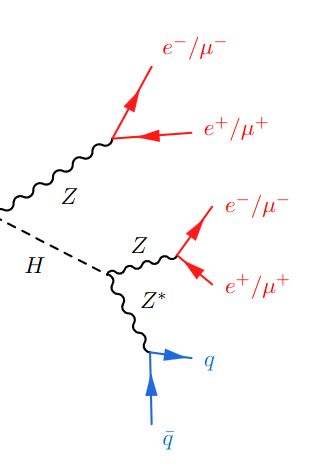
\includegraphics[scale=0.3]{lllljjFD.png}
        \captionof{figure}{$\textcolor{red}{llll}\textcolor{NavyBlue}{jj}$ decay.}
        \label{lllljjFD}
    \end{minipage}
    \end{table}
    %%%%%%%%%%%%%%%%%%%%%%
    \begin{table}[ht]
    \begin{minipage}[h]{0.7\textwidth}
        \underline{$Z_1(\textcolor{red}{ll})Z_2(\textcolor{red}{ll})Z_3(\textcolor{Green}{\nu\nu})$ Signature}    
        \begin{itemize}
            \setlength\itemsep{-0.4em}
            \item Two pairs of high-momentum leptons of same flavor and opposite sign;
            \item Both of dilepton masses, $\boldsymbol{m_{ll_1}}$ and $\boldsymbol{m_{ll_2}}$, around the $Z$ mass (91~GeV), as the four leptons come from on-shell $Z$ bosons;
            \item First dilepton recoil mass, $\boldsymbol{m^{\mbox{rec}}_{ll_1}}$, around the Higgs mass (125~GeV);
            \item High missing energy due to the presence of neutrinos.
        \end{itemize}
    \end{minipage}
    \begin{minipage}[h]{0.3\textwidth}
        \centering
        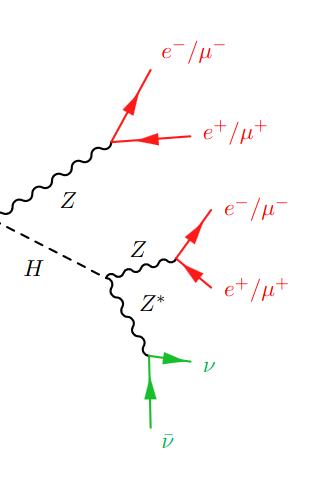
\includegraphics[scale=0.3]{llllvvFD.png}
        \captionof{figure}{$\textcolor{red}{llll}\textcolor{Green}{\nu\nu}$ decay.}
        \label{llllvvFD}
    \end{minipage}
    \end{table}
    %%%%%%%%%%%%%%%%%%%%%

    \noindent
    For the two previous channels, we distinguish $Z_1$ and $Z_2$ with the dilepton recoil masses. When reconstructing two on-shell leptonic $Z$ bosons, we compute the associated dilepton recoil masses and associate the closest one to 125 GeV to $Z_1$ and vice versa.
    
	\subsubsection[Final States With One On-Shell and One Off-Shell Leptonic $Z$ Bosons]{Final States With One On-Shell and One Off-Shell Leptonic \boldmath$Z$ Bosons}
    This section concerns the channels listed in (\ref{1OnShell1OffShell}) generally referred to as $$Z_1(\textcolor{red}{ll})Z_2(xx)Z_3(\textcolor{red}{ll}) \;\mbox{and}\; Z_1(xx)Z_2(\textcolor{red}{ll})Z_3(\textcolor{red}{ll})$$ Their signatures are introduced below.
    %%%%%%%%%%%%%%%%%%%%%%
    \begin{table}[ht]
    \begin{minipage}[h]{0.6\textwidth}
        \underline{$Z_1(\textcolor{red}{ll})Z_2(\textcolor{NavyBlue}{jj})Z_3(\textcolor{red}{ll})$ and $Z_1(\textcolor{NavyBlue}{jj})Z_2(\textcolor{red}{ll})Z_3(\textcolor{red}{ll})$ Common Signature}
        \begin{itemize}
            \setlength\itemsep{-0.4em}
            \item One pair of high-momentum leptons of same flavor and opposite sign with associated dilepton mass, $\boldsymbol{m_{ll}}$, around the $Z$ mass (91 GeV), as it comes from an on-shell $Z$ boson;
            \item One pair of low-momentum leptons of same flavor and opposite sign with associated mass, $\boldsymbol{m_{ll_3}}$, around 30~GeV as it comes from an off-shell $Z$ boson;
            \item Dijet mass, $\boldsymbol{m_{jj}}$, around the $Z$ mass (91 GeV), as the dijet comes from an on-shell $Z$ boson;
            \item Low missing energy as there are no neutrinos.
        \end{itemize}
    \end{minipage}
    \begin{minipage}[h]{0.4\textwidth}
        \centering
        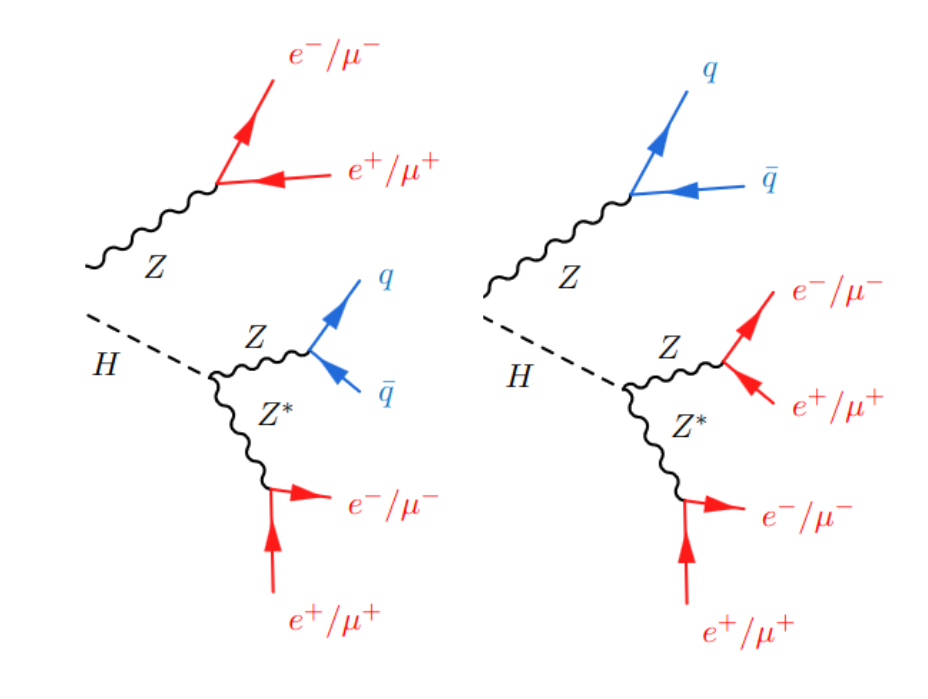
\includegraphics[scale=0.21]{lljjllFD_jjllllFD.png}
        \captionof{figure}[$\textcolor{red}{ll}\textcolor{NavyBlue}{jj}\textcolor{red}{ll}$ decay and $\textcolor{NavyBlue}{jj}\textcolor{red}{llll}$ decay.]
        {$\textcolor{red}{ll}\textcolor{NavyBlue}{jj}\textcolor{red}{ll}$ decay (left) and $\textcolor{NavyBlue}{jj}\textcolor{red}{llll}$ decay (right).}
        \label{lljjllFD_jjllllFD}
    \end{minipage}
    \end{table}
    %%%%%%%%%%%%%%%%%%%%%%
    \newpage
    \begin{table}[ht]
    \begin{minipage}[h]{0.6\textwidth}
        \underline{$Z_1(\textcolor{red}{ll})Z_2(\textcolor{Green}{\nu\nu})Z_3(\textcolor{red}{ll})$ and $Z_1(\textcolor{Green}{\nu\nu})Z_2(\textcolor{red}{ll})Z_3(\textcolor{red}{ll})$ Common Signature}
        \begin{itemize}
        \setlength\itemsep{-0.4em}
            \item One pair of high-momentum leptons of same flavor and opposite sign with associated mass, $\boldsymbol{m_{ll}}$, around the $Z$ mass (91 GeV), as it comes from an on-shell $Z$ boson;
            \item One pair of low-momentum leptons of same flavor and opposite sign with associated mass, $\boldsymbol{m_{ll_3}}$, around 30~GeV as it comes from an off-shell $Z$ boson;
            \item High missing energy due to the presence of neutrinos.
        \end{itemize}
    \end{minipage}
    \begin{minipage}[h]{0.4\textwidth}
        \centering
        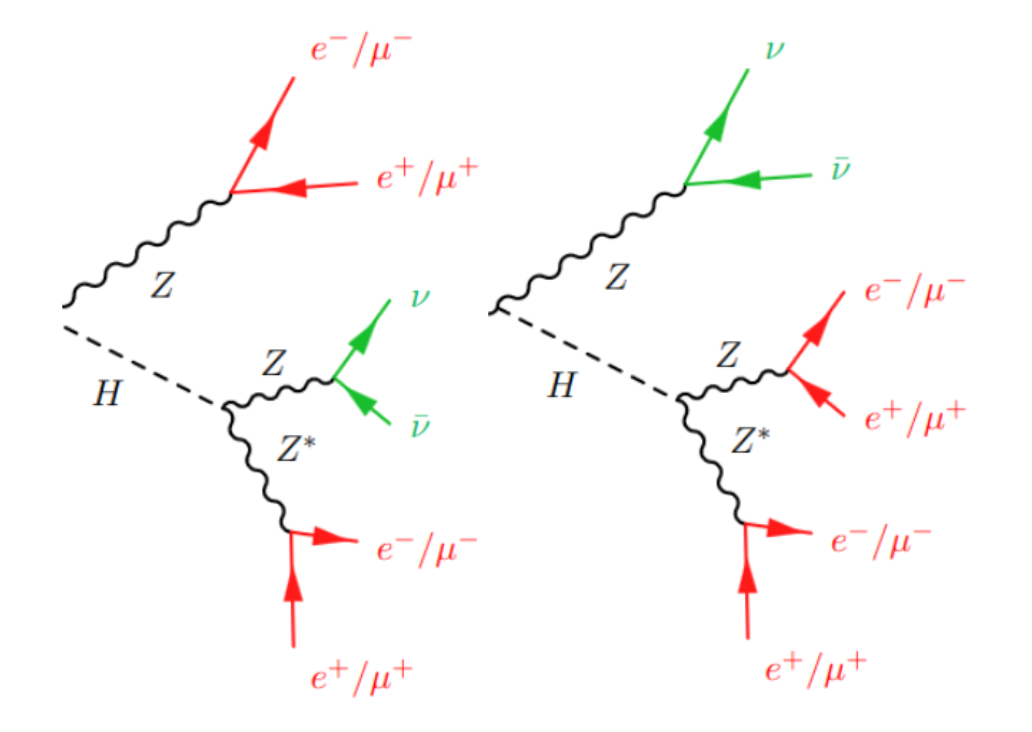
\includegraphics[scale=0.18]{llvvllFD_vvllllFD.png}
        \captionof{figure}[$\textcolor{red}{ll}\textcolor{Green}{\nu\nu}\textcolor{red}{ll}$ decay and $\textcolor{Green}{\nu\nu}\textcolor{red}{llll}$ decay.]
        {$\textcolor{red}{ll}\textcolor{Green}{\nu\nu}\textcolor{red}{ll}$ decay (left) and $\textcolor{Green}{\nu\nu}\textcolor{red}{llll}$ decay (right).}
        \label{llvvllFD_vvllllFD}
    \end{minipage}
    \end{table}
    %%%%%%%%%%%%%%%%%%%%%%
    \noindent
    Note that for the four previous channels, the two on-shell $Z$ bosons ($Z_1$ and $Z_2$) are not distinguished; the only on-shell leptonic Z considered may be reconstructed from dileptons coming from $Z_1$ as well as dileptons coming from $Z_2$. This is why the on-shell dilepton mass is called $m_{ll}$ in this case, not $m_{ll_1}$ or $m_{ll_2}$.  They will be distinguished later on by using the recoil masses.
 
	\subsection{Background Processes} \label{Background}
    Alongside the signal channels ($ZH,H(ZZ^*)$), the analysis is applied on other channels which are considered background. The background channels that were selected are the channels that are susceptible to host two pairs of two leptons similar to the pairs coming from $Z$ bosons; they can therefore be confused with $ZH,H(ZZ^*)$ with four leptons in the final state. These background channels are:
    \begin{itemize}
        \setlength\itemsep{-0.4em}
        \item $ee\rightarrow ZZ$;
        \item $ee\rightarrow ZH$ with $Z(\mu\mu,ee)$ decays and non $H(ZZ^*)$ Higgs decays ($H(WW)$, $H(\mu\mu)$, $H(qq)$, $H(\tau\tau)$, $H(Z\gamma)$).
    \end{itemize}
    Other backgrounds were considered as well:
    \begin{itemize}
        \setlength\itemsep{-0.4em}
        \item $ee\rightarrow WW$;
        \item $ee\rightarrow ZH$ with $Z(\mu\mu,ee)H(gg,\gamma\gamma)$;
        \item $ee\rightarrow ZH$ with $Z(\nu\nu)$ decays and non $H(ZZ^*)$ Higgs decays ($H(WW)$, $H(\mu\mu)$, $H(qq)$, $H(\tau\tau)$, $H(Z\gamma)$, $H(gg)$, $H(\gamma\gamma)$).
    \end{itemize}
    The latter background channels ($ZH,Z(\nu\nu)$ with non $H(ZZ^*)$ decays and $ZH,Z(\mu\mu,ee)H(\gamma\gamma)$) vanish completely after a pre-selection which requires two leptonic $Z$ bosons. However, this preselection keeps some contamination coming from $WW$ and $Z(\mu\mu,ee)H(gg)$ backgrounds (see section \ref{Results}).\\
    $ee\rightarrow WW$ and $ee\rightarrow ZZ$ Feynman diagrams are shown in Figure \ref{ZZWWFD}.
    \begin{figure}[h]
        \centering
        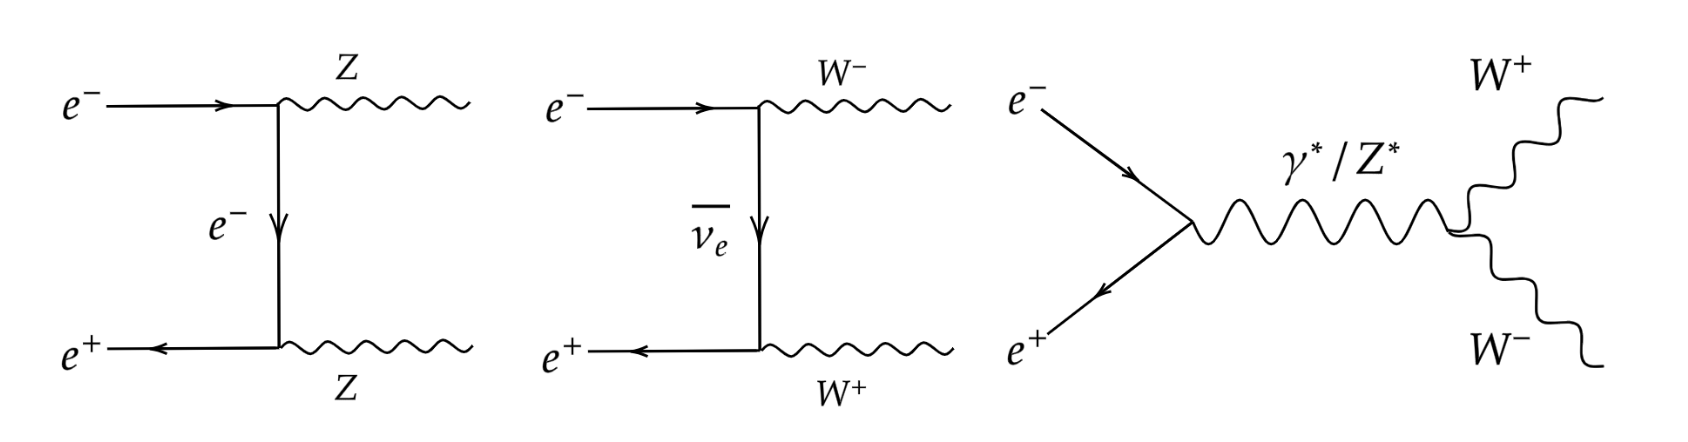
\includegraphics[scale=0.2]{ZZWWFD.png}
        \caption[Feynman diagrams of $ZZ$ and $WW$\\backgrounds at lowest order.]
        {Feynman diagrams of $ZZ$ (left) and $WW$ (centre and right)\\backgrounds at lowest order.}
        \label{ZZWWFD}
    \end{figure}

    \newpage
	\section{Results and Discussion} \label{Results}
    This section is dedicated to the results of the data analysis. The initial numbers of events of signal and background are given in table \ref{InitialNEvents}; we can see that the most dominant backgrounds are $ee\rightarrow ZZ$ and $ee\rightarrow WW$ events whose numbers are two and three orders of magnitude higher than the number of signal events.
    \begin{table}[h!]
        \centering
        \begin{adjustbox}{width=1\textwidth}
        \begin{tabular}{|c|c|c|c|c|c|c|c|c|c|}
            \hline
             \multirow{2}*{} & Signal &  \multicolumn{8}{c|}{Background} \\
             \cline{2-10}
              & $ZH(ZZ^*)$ & $ZH(WW)$ & $ZH(\mu\mu)$ & $ZH(qq)$ & $ZH(\tau\tau)$ & $ZH(Z\gamma)$ & $ZH(gg)$ & $ZZ$ & $WW$ \\
             \hline
             \thead{Number\\of Events} & $\sim 26000$ & $\sim 15000$ & $\sim 15$ & $\sim 42600$ & $\sim 4400$ & $\sim 100$ & $\sim 5700$ & $\sim 68\;10^5$ & $\sim 82\;10^6$ \\
             \hline
             \thead{Cross Section\\$[$pb$]$} & $\sim 5.4\;10^{-3}$ & $\sim 3\;10^{-3}$ & $\sim 3\;10^{-6}$ & $\sim 8.5\;10^{-3}$ & $\sim 8.7\;10^{-4}$ & $\sim 2\;10^{-5}$ & $\sim 1.1\;10^{-3}$ & $\sim 1.4$ & $\sim 16$ \\
             \hline
        \end{tabular}
        \end{adjustbox}
        \caption{Number of considered signal and background events with associated cross section at $\sqrt{s}=240$ GeV and $L=5$ ab$^{-1}$.}
        \label{InitialNEvents}
    \end{table}
    
    \subsection{Rectangular Cuts} \label{RectangularCuts}
    This subsection takes over the results obtained by applying rectangular cuts on kinematic variables in an attempt to reduce 
    the background.\\\\
    Before applying any cut, we make a preselection, called Sel 0$_{A,B}$, which requires two leptonic $Z$ bosons in the final state: two on-shell leptonic $Z$ bosons for the $Z_1(\textcolor{red}{ll})Z_2(\textcolor{red}{ll})Z_3(xx)$ channels (listed in  (\ref{2OnShell})) and one on-shell and one off-shell leptonic $Z$ bosons for the $Z_1(\textcolor{red}{ll})Z_3(xx)Z_1(\textcolor{red}{ll})$ and $Z_1(xx)Z_2(\textcolor{red}{ll})Z_3(\textcolor{red}{ll})$ channels (listed in (\ref{1OnShell1OffShell})). This preselection gives way to a series of rectangular cuts whose purpose is to reduce the background while keeping as much signal as possible. The results of these cuts are presented in cutflow tables and the variables' distributions used for the selections are to be found in appendix \ref{CutflowVariables}.

    \subsubsection[Common Cuts to Final States With Two On-Shell Leptonic $Z$ Bosons]{Common Cuts to Final States With Two On-Shell Leptonic \boldmath$Z$ Bosons}
    When considering two on-shell leptonic $Z$ bosons in the final state, a second cut is common to $Z_1(\textcolor{red}{ll})Z_2(\textcolor{red}{ll})Z_3(xx)$ channels in addition to the preselection (Sel 0$_A$) which requires two leptonic on-shell $Z$ bosons. This second cut is applied on the dilepton masses requiring them to be around 91 GeV (Sel 1$_A$) The missing energy is used afterwards to distinguish $xx=\textcolor{NavyBlue}{jj}$ and $xx=\textcolor{Green}{\nu\nu}$ ($E^{\mbox{miss}}<8$ for $xx=\textcolor{NavyBlue}{jj}$ and $E^{\mbox{miss}}>8$ for $xx=\textcolor{Green}{\nu\nu}$). The cutflow of the common selections is presented in Table \ref{Cutflowllllxx}.
    \begin{table}[h!]
        \centering
        \begin{adjustbox}{width=1\textwidth}
        \begin{tabular}{|c|c|c|c|c|c|c|c|c|c|}
            \hline
            \multicolumn{10}{p{1\textwidth}}{Variables} \\
            \hline
            \multicolumn{10}{p{1\textwidth}}{$m_{ll_1}$ and $m_{ll_2}$: mass of the dilepton associated to $Z_1$ and $Z_2$ respectively} \\
            \multicolumn{10}{p{1\textwidth}}{$E^{\mbox{miss}}$: missing energy} \\
            \hline
             & Signal & \multicolumn{8}{c|}{Background} \\
             \hline
            Selection & \thead{$ZH(ZZ^*)$} & \thead{$ZH(WW)$} & \thead{$ZH(\mu\mu)$} & \thead{$ZH(qq)$} & \thead{$ZH(\tau\tau)$} & \thead{$ZH(Z\gamma)$} & \thead{$ZH(gg)$} & \thead{$ZZ$} & \thead{$WW$} \\
            \hline
            \thead{Two $Z(\textcolor{red}{ll})$ \& no $Z^*(\textcolor{red}{ll})$ \\ (Sel $0_A$)} & \thead{113.6\\$\pm0.5$} & \thead{181\\$\pm2$} & \thead{7.56\\$\pm0.01$} & \thead{25\\$\pm1$} & \thead{59.4\\$\pm0.6$} & \thead{5.76\\$\pm0.03$} & \thead{0.007\\$\pm0.007$} & \thead{12196\\$\pm38$} & \thead{47\\$\pm3$} \\
            \thead{Sel $0_A$ + $m_{ll_{1,2}}\in[80,110]$ GeV \\ (Sel $1_A$)} & \thead{65.2\\$\pm0.4$} & \thead{1.0\\$\pm0.1$} & \thead{0.538\\$\pm0.003$} & \thead{0\\$\pm\delta<1$} & \thead{8.7\\$\pm0.2$} & \thead{4.63\\$\pm0.02$} & \thead{0\\$\pm\delta<0.007$} & \thead{6286\\$\pm28$} & \thead{0\\$\pm\delta<3$} \\
            \thead{Sel $1_A$ + $E^{\mbox{miss}}<8$ GeV \\ (Sel $2_{AA}$)} & \thead{46.1\\$\pm0.3$} & \thead{0.02\\$\pm0.02$} & \thead{0.498\\$\pm0.003$} & \thead{0\\$\pm\delta<1$} & \thead{0.52\\$\pm0.05$} & \thead{4.34\\$\pm0.02$} & \thead{0\\$\pm\delta<0.007$} & \thead{4817\\$\pm24$} & \thead{0\\$\pm\delta<3$} \\
            \thead{Sel $1_A$ + $E^{\mbox{miss}}>8$ GeV \\ (Sel $2_{AB}$)} & \thead{19.1\\$\pm0.2$} & \thead{1.0\\$\pm0.1$} & \thead{0.0399\\$\pm0.0009$} & \thead{0\\$\pm\delta<1$} & \thead{8.2\\$\pm0.2$} & \thead{0.289\\$\pm0.006$} & \thead{0\\$\pm\delta<0.007$} & \thead{1468\\$\pm13$} & \thead{0\\$\pm\delta<3$} \\
            \hline
        \end{tabular}
        \end{adjustbox}
        \caption[Cutflow of the $Z_1(\textcolor{red}{ll})Z_2(\textcolor{red}{ll})Z_3(xx)$ channels.]%
        {Cutflow of the $Z_1(\textcolor{red}{ll})Z_2(\textcolor{red}{ll})Z_3(xx)$ channels.}
        \label{Cutflowllllxx}
    \end{table}

    \subsubsection[Common Cuts to Final States With One On-Shell and One Off-Shell Leptonic $Z$ Bosons]{Common Cuts to Final States With One On-Shell and One Off-Shell Leptonic \boldmath$Z$ Bosons}
    As previously, some selections are common to $Z_1(\textcolor{red}{ll})Z_2(xx)Z_3(\textcolor{red}{ll})$ and $Z_1(xx)Z_2(\textcolor{red}{ll})Z_3(\textcolor{red}{ll})$: Sel 0$_B$, which requires one on-shell and one off-shell leptonic $Z$ bosons, Sel 1$_B$ and Sel 2$_B$ which restrict the dilepton masses. From then, we discriminate between $xx=\textcolor{NavyBlue}{jj}$ and $xx=\textcolor{Green}{\nu\nu}$ using the missing energy.
    The cutflow associated to these first selections is presented in Table \ref{Cutflowllxxll}.
    \begin{table}[h!]
        \centering
        \begin{adjustbox}{width=1\textwidth}
        \begin{tabular}{|c|c|c|c|c|c|c|c|c|c|}
            \hline
            \multicolumn{10}{p{1\textwidth}}{Variables} \\
            \hline
            \multicolumn{10}{p{1\textwidth}}{$m_{ll}$: mass of the dilepton associated to the on-shell $Z$ ($Z_1$ or $Z_2$)} \\
            \multicolumn{10}{p{1\textwidth}}{$m_{ll_3}$: mass of the dilepton associated to the off-shell $Z$ ($Z_3$)} \\
            \multicolumn{10}{p{1\textwidth}}{$E^{\mbox{miss}}$: missing energy} \\
            \hline
             & Signal & \multicolumn{8}{c|}{Background} \\
             \hline
            Selection & \thead{$ZH(ZZ^*)$} & \thead{$ZH(WW)$} & \thead{$ZH(\mu\mu)$} & \thead{$ZH(qq)$} & \thead{$ZH(\tau\tau)$} & \thead{$ZH(Z\gamma)$} & \thead{$ZH(gg)$} & \thead{$ZZ$} & \thead{$WW$} \\
            \hline
            \thead{One $Z(\textcolor{red}{ll})$ \& one $Z^*(\textcolor{red}{ll})$ \\ (Sel $0_B$)} & \thead{206.8\\$\pm0.8$} & \thead{270\\$\pm2$} & \thead{5.97\\$\pm0.01$} & \thead{951\\$\pm7$} & \thead{130.5\\$\pm0.8$} & \thead{1.17\\$\pm0.01$} & \thead{5.1\\$\pm0.2$} & \thead{28340\\$\pm59$} & \thead{846\\$\pm14$} \\
            \thead{Sel $0_B$ + $m_{ll}\in[80,110]$ GeV \\ (Sel $1_B$)} & \thead{173.4\\$\pm0.7$} & \thead{246\\$\pm2$} & \thead{5.27\\$\pm0.01$} & \thead{866\\$\pm6$} & \thead{118.6\\$\pm0.8$} & \thead{1.06\\$\pm0.01$} & \thead{4.7\\$\pm0.2$} & \thead{15680\\$\pm44$} & \thead{257\\$\pm8$} \\
            \thead{Sel $1_B$ + $m_{ll_3}\in[10,40]$ GeV \\ (Sel $2_B$)} & \thead{158.2\\$\pm0.7$} & \thead{187\\$\pm2$} & \thead{0.0288\\$\pm0.0007$} & \thead{462\\$\pm4$} & \thead{76.4\\$\pm0.6$} & \thead{0.337\\$\pm0.007$} & \thead{0.77\\$\pm0.07$} & \thead{3097\\$\pm19$} & \thead{12\\$\pm2$} \\
            \thead{Sel $2_B$ + $E^{\mbox{miss}}<8$ GeV \\ (Sel $3_{BA}$)} & \thead{96.4\\$\pm0.5$} & \thead{1.4\\$\pm0.2$} & \thead{0.0268\\$\pm0.0007$} & \thead{155\\$\pm2$} & \thead{0.19\\$\pm0.03$} & \thead{0.152\\$\pm0.005$} & \thead{0.32\\$\pm0.05$} & \thead{1412\\$\pm13$} & \thead{0\\$\pm\delta<2$} \\
            \thead{Sel $2_B$ + $E^{\mbox{miss}}>8$ GeV \\ (Sel $3_{BB}$)} & \thead{61.8\\$\pm0.4$} & \thead{186\\$\pm2$} & \thead{0.0020\\$\pm0.0002$} & \thead{307\\$\pm4$} & \thead{76.2\\$\pm0.6$} & \thead{0.185\\$\pm0.005$} & \thead{0.45\\$\pm0.06$} & \thead{1685\\$\pm14$} & \thead{12\\$\pm2$} \\
            \hline
        \end{tabular}
        \end{adjustbox}
        \caption{First selections on the $Z_1(\textcolor{red}{ll})Z_2(xx)Z_3(\textcolor{red}{ll})$ and $Z_1(xx)Z_2(\textcolor{red}{ll})Z_3(\textcolor{red}{ll})$ channels.}
        \label{Cutflowllxxll}
    \end{table}

    \noindent
    \subsubsection[$Z_1(\textcolor{red}{ll})Z_2(\textcolor{red}{ll})Z_3(\textcolor{NavyBlue}{jj})$ and $Z_1(\textcolor{red}{ll})Z_2(\textcolor{red}{ll})Z_3(\textcolor{Green}{\nu\nu})$ Cutflow]{\boldmath$Z_1(\textcolor{red}{ll})Z_2(\textcolor{red}{ll})Z_3(\textcolor{NavyBlue}{jj})$ and $Z_1(\textcolor{red}{ll})Z_2(\textcolor{red}{ll})Z_3(\textcolor{Green}{\nu\nu})$ Cutflow}
    The cutflow of $Z_1(\textcolor{red}{ll})Z_2(\textcolor{red}{ll})Z_3(\textcolor{NavyBlue}{jj})$ is presented in Table \ref{Cutflowlllljj} in which the most dominant source of background after all selections is emphasized in bold. The error on the number of events is a statistical error due to the finite number of Monte Carlo events.\\
    Among all considered decay channels, $Z_1(\textcolor{red}{ll})Z_2(\textcolor{red}{ll})Z_3(\textcolor{NavyBlue}{jj})$ stands out as being the purest channel with only $ZZ$ events as dominant background events after the final selection (Sel $4_{AA}$).\\\\
    \underline{Note}: for this channel, a cut was applied on $m^{\mbox{rec}}_{ll_2+\gamma}$, which is the recoil mass of the four-vector obtained by summing the $Z_2$ four-vector and the highest-energy photon four-vector. Its purpose was to diminish the $ZZ$ background and it worked better than cutting on $m^{\mbox{rec}}_{ll_2}$ which is the recoil mass of the $Z_2$ four-vector alone, although it is not clear why.
    \begin{table}[h!]
        \centering
        \begin{adjustbox}{width=1\textwidth}
        \begin{tabular}{|c|c|c|c|c|c|c|c|c|c|}
            \hline
            \multicolumn{10}{p{1\textwidth}}{Variables} \\
            \hline
            \multicolumn{10}{p{1\textwidth}}{$E^\gamma$: energy of the highest-energy photon} \\
            \multicolumn{10}{p{1\textwidth}}{$m^{\mbox{rec}}_{ll_2+\gamma}$: recoil mass of the four-vector obtained by the summing the $Z_2$ four-vector and the highest-energy photon four-vector} \\
            \hline
             & Signal & \multicolumn{8}{c|}{Background} \\
             \hline
            Selection & \thead{$ZH(ZZ^*)$} & \thead{$ZH(WW)$} & \thead{$ZH(\mu\mu)$} & \thead{$ZH(qq)$} & \thead{$ZH(\tau\tau)$} & \thead{$ZH(Z\gamma)$} & \thead{$ZH(gg)$} & \thead{\boldmath$ZZ$} & \thead{$WW$} \\
            \hline
            \thead{Sel $2_{AA}$ + $E^\gamma<20$ GeV \\ (Sel $3_{AA}$)} & \thead{45.1\\$\pm0.3$} & \thead{0.02\\$\pm0.02$} & \thead{0.204\\$\pm0.002$} & \thead{0\\$\pm<1$} & \thead{0.43\\$\pm0.05$} & \thead{0.135\\$\pm0.004$} & \thead{0\\$\pm\delta<0.007$} & \thead{3539\\$\pm21$} & \thead{0\\$\delta<3$} \\
            \thead{Sel $3_{AA}$ + $m^{\mbox{rec}}_{ll_2+\gamma}>115$ GeV \\ (Sel $4_{AA}$)} & \thead{41.3\\$\pm0.3$} & \thead{0.02\\$\pm0.02$} & \thead{0.0160\\$\pm0.0005$} & \thead{0\\$\pm\delta<1$} & \thead{0.32\\$\pm0.04$} & \thead{0.030\\$\pm0.002$} & \thead{0\\$\pm\delta<0.007$} & \thead{29\\$\pm2$} & \thead{0\\$\pm\delta<3$} \\
            \hline
        \end{tabular}
        \end{adjustbox}
        \caption[Cutflow of the $Z_1(\textcolor{red}{ll})Z_2(\textcolor{red}{ll})Z_3(\textcolor{NavyBlue}{jj})$ channel.]%
        {Cutflow of the $Z_1(\textcolor{red}{ll})Z_2(\textcolor{red}{ll})Z_3(\textcolor{NavyBlue}{jj})$ channel.}
        \label{Cutflowlllljj}
    \end{table}

    \noindent
    The cutflow of $Z_1(\textcolor{red}{ll})Z_2(\textcolor{red}{ll})Z_3(\textcolor{Green}{\nu\nu})$ is presented in Table \ref{Cutflowllllvv}. In addition to background coming from $ZZ$, this channel encounters $ZH(\tau\tau)$ as a remaining abundant background after the final selection (Sel $4_{AB}$).
    \begin{table}[h!]
        \centering
        \begin{adjustbox}{width=1\textwidth}
        \begin{tabular}{|c|c|c|c|c|c|c|c|c|c|}
            \hline
            \multicolumn{10}{p{1\textwidth}}{Variables} \\
            \hline
            \multicolumn{10}{p{1\textwidth}}{$m^{\mbox{rec}}_{ll_2}$: recoil mass of the dilepton associated to $Z_2$} \\
            \hline
             & Signal & \multicolumn{8}{c|}{Background} \\
             \hline
            Selection & \thead{$ZH(ZZ^*)$} & \thead{$ZH(WW)$} & \thead{$ZH(\mu\mu)$} & \thead{$ZH(qq)$} & \thead{\boldmath$ZH(\tau\tau)$} & \thead{$ZH(Z\gamma)$} & \thead{$ZH(gg)$} & \thead{\boldmath$ZZ$} & \thead{$WW$} \\
            \hline
            \thead{Sel $2_{AB}$ + $m^{\mbox{rec}}_{ll_2}\in[125,150]$ GeV \\ (Sel $3_{AB}$)} & \thead{16.1\\$\pm0.2$} & \thead{0.7\\$\pm0.1$} & \thead{0.0267\\$\pm0.0007$} & \thead{0\\$\pm\delta<1$} & \thead{6.8\\$\pm0.2$} & \thead{0.264\\$\pm0.006$} & \thead{0\\$\pm\delta<0.007$} & \thead{577\\$\pm8$} & \thead{0\\$\pm\delta<3$} \\
            %\thead{Sel $3_{AB}$ + $m^{\mbox{rec}}_{ll_2}\in[125,150]$ GeV \\ (Sel $4_{AB}$)} & \thead{11.0\\$\pm0.2$} & \thead{0.36\\$\pm0.08$} & \thead{0.0093\\$\pm0.0004$} & \thead{0\\$\pm\delta<1$} & \thead{5.6\\$\pm0.2$} & \thead{0.059\\$\pm0.003$} & \thead{0\\$\pm\delta<0.007$} & \thead{201\\$\pm5$} & \thead{0\\$\pm\delta<3$} \\
            \hline
        \end{tabular}
        \end{adjustbox}
        \caption[Cutflow of the $Z_1(\textcolor{red}{ll})Z_2(\textcolor{red}{ll})Z_3(\textcolor{Green}{\nu\nu})$ channel.]%
        {Cutflow of the $Z_1(\textcolor{red}{ll})Z_2(\textcolor{red}{ll})Z_3(\textcolor{Green}{\nu\nu})$ channel.}
        \label{Cutflowllllvv}
    \end{table}
    
    \noindent
    \newpage
    \subsubsection[$Z_1(\textcolor{red}{ll})Z_2(\textcolor{NavyBlue}{jj})Z_3(\textcolor{red}{ll})$ and $Z_1(\textcolor{NavyBlue}{jj})Z_2(\textcolor{red}{ll})Z_3(\textcolor{red}{ll})$ Cutflow]{\boldmath$Z_1(\textcolor{red}{ll})Z_2(\textcolor{NavyBlue}{jj})Z_3(\textcolor{red}{ll})$ and $Z_1(\textcolor{NavyBlue}{jj})Z_2(\textcolor{red}{ll})Z_3(\textcolor{red}{ll})$ Cutflow}
    In order to distinguish $Z_1(\textcolor{red}{ll})Z_2(\textcolor{NavyBlue}{jj})Z_3(\textcolor{red}{ll})$ and $Z_1(\textcolor{NavyBlue}{jj})Z_2(\textcolor{red}{ll})Z_3(\textcolor{red}{ll})$, we compare the recoil mass of the on-shell leptonic $Z$ boson ($\boldsymbol{m^{\mbox{rec}}_{ll}}$) to the recoil mass of the dijet ($\boldsymbol{m^{\mbox{rec}}_{jj}}$); the one being closer to 125~GeV would be associated to $Z_1$. To do so, we introduce the discriminant:
    \begin{equation}
        \Delta=|125\;\mbox{GeV}-m^{\mbox{rec}}_{jj}|-|125\;\mbox{GeV}-m^{\mbox{rec}}_{ll}|
    \end{equation} 
    $\Delta>0$ for $Z_1(\textcolor{red}{ll})Z_2(\textcolor{NavyBlue}{jj})Z_3(\textcolor{red}{ll})$ and $\Delta<0$ for $Z_1(\textcolor{NavyBlue}{jj})Z_2(\textcolor{red}{ll})Z_3(\textcolor{red}{ll})$. Their cutflows are presented in Table~\ref{Cutflowlljjll} and Table \ref{Cutflowjjllll}.

    \begin{table}[h!]
        \centering
        \begin{adjustbox}{width=1\textwidth}
        \begin{tabular}{|c|c|c|c|c|c|c|c|c|c|}
            \hline
            \multicolumn{10}{p{1\textwidth}}{Variables} \\
            \hline
            \multicolumn{10}{p{1\textwidth}}{$m_{jj}$: mass of the dijet} \\
            \multicolumn{10}{p{1\textwidth}}{$m^{\mbox{rec}}_{ll_3}$: recoil mass of the dilepton associated to $Z_3$} \\
            \multicolumn{10}{p{1\textwidth}}{$m^{\mbox{rec}}_{jj+ll_3}$: recoil mass of the four-vector obtained by summing the dijet four-vector and the $Z_3$ four-vector} \\
            \hline
             & Signal & \multicolumn{8}{c|}{Background} \\
             \hline
            Selection & \thead{$ZH(ZZ^*)$} & \thead{$ZH(WW)$} & \thead{$ZH(\mu\mu)$} & \thead{\boldmath$ZH(qq)$} & \thead{$ZH(\tau\tau)$} & \thead{$ZH(Z\gamma)$} & \thead{$ZH(gg)$} & \thead{\boldmath$ZZ$} & \thead{$WW$} \\
            \hline
            \thead{Sel $3_{BA}$ + $\Delta>0$ \\ (Sel $4_{BAA}$)} & \thead{51.5\\$\pm0.4$} & \thead{1.3\\$\pm0.2$} & \thead{0.0248\\$\pm0.0007$} & \thead{137\\$\pm2$} & \thead{0.19\\$\pm0.03$} & \thead{0.127\\$\pm0.004$} & \thead{0.21\\$\pm0.04$} & \thead{741\\$\pm9$} & \thead{0\\$\pm\delta<2$} \\
            \thead{Sel $4_{BAA}$ + $m_{jj}\in[80,110]$ GeV \\ (Sel $5_{BAA}$)} & \thead{44.8\\$\pm0.3$} & \thead{0.30\\$\pm0.07$} & \thead{0.0005\\$\pm0.0001$} & \thead{101\\$\pm2$} & \thead{0.011\\$\pm0.008$} & \thead{0.064\\$\pm0.003$} & \thead{0.20\\$\pm0.04$} & \thead{23\\$\pm2$} & \thead{0\\$\pm\delta<2$} \\
            \thead{Sel $5_{BAA}$ + $m^{\mbox{rec}}_{ll_3}\in[190,215]$ GeV \\ (Sel $6_{BAA}$)} & \thead{40.6\\$\pm0.3$} & \thead{0.07\\$\pm0.04$} & \thead{$0.0005$\\$\pm0.0001$} & \thead{40\\$\pm1$} & \thead{0.005\\$\pm0.005$} & \thead{0.024\\$\pm0.002$} & \thead{0.04\\$\pm0.02$} & \thead{10\\$\pm1$} & \thead{0\\$\pm\delta<2$} \\
            \thead{Sel $6_{BAA}$ + $m^{\mbox{rec}}_{jj+ll_3}\in[80,110]$ GeV \\ (Sel $7_{BAA}$)} & \thead{40.1\\$\pm0.3$} & \thead{0.07\\$\pm0.03$} & \thead{0.0005\\$\pm0.0001$} & \thead{34\\$\pm1$} & \thead{0.005\\$\pm0.005$} & \thead{0.022\\$\pm0.002$} & \thead{0.04\\$\pm0.02$} & \thead{8\\$\pm1$} & \thead{0\\$\pm\delta<2$} \\
            \hline
        \end{tabular}
        \end{adjustbox}
        \caption{Cutflow of the $Z_1(\textcolor{red}{ll})Z_2(\textcolor{NavyBlue}{jj})Z_3(\textcolor{red}{ll})$ channel.}
        \label{Cutflowlljjll}
    \end{table}

    \begin{table}[h!]
        \centering
        \begin{adjustbox}{width=1\textwidth}
        \begin{tabular}{|c|c|c|c|c|c|c|c|c|c|}
            \hline
            \multicolumn{10}{p{1\textwidth}}{Variables} \\
            \hline
            \multicolumn{10}{p{1\textwidth}}{$m_{jj}$: mass of the dijet} \\
            \multicolumn{10}{p{1\textwidth}}{$m^{\mbox{rec}}_{ll_3}$: recoil mass of the dilepton associated to $Z_3$} \\
             \multicolumn{10}{p{1\textwidth}}{$m_{ll_2+ll_3}$: mass of the four-vector obtained by summing the $Z_2$ four-vector and the $Z_3$ four-vector} \\
            \hline
             & Signal & \multicolumn{8}{c|}{Background} \\
             \hline
            Selection & \thead{$ZH(ZZ^*)$} & \thead{$ZH(WW)$} & \thead{$ZH(\mu\mu)$} & \thead{\boldmath$ZH(qq)$} & \thead{$ZH(\tau\tau)$} & \thead{$ZH(Z\gamma)$} & \thead{$ZH(gg)$} & \thead{\boldmath$ZZ$} & \thead{$WW$} \\
            \hline
            \thead{Sel $3_{BA}$ + $\Delta<0$ \\ (Sel $4_{BAB}$)} & \thead{44.9\\$\pm0.4$} & \thead{0.11\\$\pm0.05$} & \thead{0.0020\\$\pm0.0002$} & \thead{18.3\\$\pm0.8$} & \thead{0\\$\pm\delta<0.03$} & \thead{0.024\\$\pm0.002$} & \thead{0.11\\$\pm0.03$} & \thead{663\\$\pm9$} & \thead{0\\$\pm\delta<2$} \\
            \thead{Sel $4_{BAB}$ + $m_{jj}\in[80,110]$ GeV \\ (Sel $5_{BAB}$)} & \thead{42.4\\$\pm0.4$} & \thead{0.11\\$\pm0.05$} & \thead{$2.8\;10^{-4}$\\$\pm0.8\;10^{-4}$} & \thead{16.0\\$\pm0.8$} & \thead{0\\$\pm\delta<0.03$} & \thead{0.017\\$\pm0.002$} & \thead{0.09\\$\pm0.03$} & \thead{87\\$\pm3$} & \thead{0\\$\pm\delta<2$} \\
            \thead{Sel $5_{BAB}$ + $m^{\mbox{rec}}_{ll_3}\in[195,215]$ GeV \\ (Sel $6_{BAB}$)} & \thead{38.3\\$\pm0.4$} & \thead{0.02\\$\pm0.02$} & \thead{$1.2\;10^{-4}$\\$\pm0.5\;10^{-4}$} & \thead{4.4\\$\pm0.4$} & \thead{0\\$\pm\delta<0.03$} & \thead{0.006\\$\pm0.001$} & \thead{0.02\\$\pm0.01$} & \thead{9\\$\pm1$} & \thead{0\\$\pm\delta<2$} \\
            \hline
        \end{tabular}
        \end{adjustbox}
        \caption{Cutflow of the $Z_1(\textcolor{NavyBlue}{jj})Z_2(\textcolor{red}{ll})Z_3(\textcolor{red}{ll})$ channel.}
        \label{Cutflowjjllll}
    \end{table}

    \noindent
    \subsubsection[$Z_1(\textcolor{red}{ll})Z_2(\textcolor{Green}{\nu\nu})Z_3(\textcolor{red}{ll})$ and $Z_1(\textcolor{Green}{\nu\nu})Z_2(\textcolor{red}{ll})Z_3(\textcolor{red}{ll})$ Cutflow]{\boldmath$Z_1(\textcolor{red}{ll})Z_2(\textcolor{Green}{\nu\nu})Z_3(\textcolor{red}{ll})$ and $Z_1(\textcolor{Green}{\nu\nu})Z_2(\textcolor{red}{ll})Z_3(\textcolor{red}{ll})$ Cutflow}
    To differentiate $Z_1(\textcolor{red}{ll})Z_2(\textcolor{Green}{\nu\nu})Z_3(\textcolor{red}{ll})$ and $Z_1(\textcolor{Green}{\nu\nu})Z_2(\textcolor{red}{ll})Z_3(\textcolor{red}{ll})$, we use the recoil mass of the on-shell $Z$ boson ($\boldsymbol{m^{\mbox{rec}}_{ll}}$) as it should be around 125 GeV for $Z_1(\textcolor{red}{ll})Z_2(\textcolor{Green}{\nu\nu})Z_3(\textcolor{red}{ll})$. The associated cutflows are presented in tables \ref{Cutflowllvvll} and \ref{Cutflowvvllll}.
    
    \begin{table}[h!]
        \centering
        \begin{adjustbox}{width=1\textwidth}
        \begin{tabular}{|c|c|c|c|c|c|c|c|c|c|}
            \hline
            \multicolumn{10}{p{1\textwidth}}{Variables} \\
            \hline
            \multicolumn{10}{p{1\textwidth}}{$m^{\mbox{rec}}_{ll}$: recoil mass of the dilepton associated to the on-shell $Z$ ($Z_1$ or $Z_2$).} \\
            \hline
             & Signal & \multicolumn{8}{c|}{Background} \\
             \hline
            Selection & \thead{$ZH(ZZ^*)$} & \thead{\boldmath$ZH(WW)$} & \thead{$ZH(\mu\mu)$} & \thead{\boldmath$ZH(qq)$} & \thead{\boldmath$ZH(\tau\tau)$} & \thead{$ZH(Z\gamma)$} & \thead{$ZH(gg)$} & \thead{\boldmath$ZZ$} & \thead{\boldmath$WW$} \\
            \hline
            \thead{Sel $3_{BB}$ + $m^{\mbox{rec}}_{ll}\in[123,127]$ GeV \\ (Sel $4_{BBA}$)} & \thead{20.3\\$\pm0.42$} & \thead{119\\$\pm1$} & \thead{$2\;10^{-5}$\\$\pm2\;10^{-5}$} & \thead{195\\$\pm3$} & \thead{49.0\\$\pm0.5$} & \thead{0.114\\$\pm0.004$} & \thead{0.29\\$\pm0.05$} & \thead{84\\$\pm3$} & \thead{1.1\\$\pm0.5$} \\
            \hline
        \end{tabular}
        \end{adjustbox}
        \caption{Cutflow of the $Z_1(\textcolor{red}{ll})Z_2(\textcolor{Green}{\nu\nu})Z_3(\textcolor{red}{ll})$ channel.}
        \label{Cutflowllvvll}
    \end{table}

    \begin{table}[h!]
        \centering
        \begin{adjustbox}{width=1\textwidth}
        \begin{tabular}{|c|c|c|c|c|c|c|c|c|c|}
            \hline
            \multicolumn{10}{p{1\textwidth}}{Variables} \\
            \hline
            \multicolumn{10}{p{1\textwidth}}{$m^{\mbox{rec}}_{ll}$: recoil mass of the dilepton associated to the on-shell $Z$ ($Z_1$ or $Z_2$)} \\
            \multicolumn{10}{p{1\textwidth}}{$E^{\mbox{miss}}$: missing energy} \\
            \multicolumn{10}{p{1\textwidth}}{$m^{\mbox{vis}}$: visible mass} \\
            \hline
             & Signal & \multicolumn{8}{c|}{Background} \\
             \hline
            Selection & \thead{$ZH(ZZ^*)$} & \thead{\boldmath$ZH(WW)$} & \thead{$ZH(\mu\mu)$} & \thead{$ZH(qq)$} & \thead{\boldmath$ZH(\tau\tau)$} & \thead{$ZH(Z\gamma)$} & \thead{$ZH(gg)$} & \thead{\boldmath$ZZ$} & \thead{$WW$} \\
            \hline
            \thead{Sel $3_{BB}$ + $m^{\mbox{rec}}_{ll}\notin[123,127]$ GeV \\ (Sel $4_{BBB}$)} & \thead{38.1\\$\pm0.4$} & \thead{67\\$\pm1$} & \thead{$0.0020$\\$\pm0.0002$} & \thead{112\\$\pm2$} & \thead{27.2\\$\pm0.4$} & \thead{0.070\\$\pm0.003$} & \thead{0.16\\$\pm0.03$} & \thead{1601\\$\pm14$} & \thead{11\\$\pm2$} \\
            \thead{Sel $4_{BBB}$ + $E^{\mbox{miss}}\in[45,55]$ GeV \\ (Sel $5_{BBB}$)} & \thead{12.3\\$\pm0.2$} & \thead{12.9\\$\pm0.5$} & \thead{$0$\\$\pm\delta<0.0002$} & \thead{0.4\\$\pm0.1$} & \thead{4.5\\$\pm0.2$} & \thead{0.0040\\$\pm0.0007$} & \thead{0\\$\pm\delta<0.03$} & \thead{161\\$\pm4$} & \thead{2.0\\$\pm0.7$} \\
            \thead{Sel $5_{BBB}$ + $m^{\mbox{vis}}<135$ GeV \\ (Sel $6_{BBB}$)} & \thead{12.0\\$\pm0.2$} & \thead{2.0\\$\pm0.2$} & \thead{$0$\\$\pm\delta<0.0002$} & \thead{0\\$\pm\delta<0.1$} & \thead{3.1\\$\pm0.1$} & \thead{0.0002\\$\pm0.0001$} & \thead{0\\$\pm\delta<0.03$} & \thead{13\\$\pm1$} & \thead{0.7\\$\pm0.4$} \\
            \hline
        \end{tabular}
        \end{adjustbox}
        \caption{Cutflow of the $Z_1(\textcolor{Green}{\nu\nu})Z_2(\textcolor{red}{ll})Z_3(\textcolor{red}{ll})$ channel.}
        \label{Cutflowvvllll}
    \end{table}
    
	\subsection[$ZH,H(ZZ^*)$ Cross Section Measurement]{\boldmath$ZH,H(ZZ^*)$ Cross Section Measurement}
    The final step of the analysis is to perform a fit using Combine, a CMS tool \cite{cms2024combine}. Performing a fit aims at finding the value of a parameter of a given model which best suits the data and comparing it to the theoretical value. Combine gives in output the signal strength $\mu=\frac{\sigma}{\sigma_{SM}}$ as the \acrshort{POI}. It is proportional to the number of signal events in the discriminating variable's distribution on which the fit is applied, the discriminating variable being a variable showing a clear separation between signal and background. The goal is to evaluate how much the variable's distribution fits the theoretical prediction of its \acrshort{PDF} depending on the POI and other parameters such as systematic uncertainties.\\\\
    \noindent
    The rectangular cuts (see section \ref{RectangularCuts}) bring out four clean channels for which we have a signal over background ratio higher than 0.5 and clear discriminating variables (see Table \ref{FitChannels}).

    \begin{table}[h!]
        \centering
        %\begin{adjustbox}{width=1\textwidth}
        \begin{tabular}{|c|c|c|c|}
            \hline
            Channel & $S/B$ & $S/\sqrt{B}$ & Discriminating Variable \\
            \hline
            $Z_1(\textcolor{red}{ll})Z_2(\textcolor{red}{ll})Z_3(\textcolor{NavyBlue}{jj})$ & $1.5\pm\delta<0.8$ & $7.9\pm\delta<2.1$ & \thead{$m^{\mbox{rec}}_{ll_1}$\\(recoil mass of $Z_1$)} \\
            $Z_1(\textcolor{red}{ll})Z_2(\textcolor{NavyBlue}{jj})Z_3(\textcolor{red}{ll})$ & $0.95\pm\delta<0.14$ & $6.2\pm\delta<0.4$ & \thead{$m_{jj+ll_3}$\\(mass of dijet+$Z_3$)} \\
            $Z_1(\textcolor{NavyBlue}{jj})Z_2(\textcolor{red}{ll})Z_3(\textcolor{red}{ll})$ & $3.1\pm\delta<1.3$ & $10.9\pm\delta<2.3$ & \thead{$m_{ll_2+ll_3}$\\(mass of $Z_2+Z_3$)} \\
            $Z_1(\textcolor{Green}{\nu\nu})Z_2(\textcolor{red}{ll})Z_3(\textcolor{red}{ll})$ & $0.75\pm\delta<0.06$ & $2.9\pm\delta<0.1$ & \thead{$m_{ll_2+ll_3}$\\(mass of $Z_2+Z_3$)} \\
            \hline
        \end{tabular}
        %\end{adjustbox}
        \caption[Channels used for the fit with their associated signal over background ratios and discriminating variables.]
        {Channels used for the fit with their associated signal over background ratios and discriminating variables.\\$S$ is the number of signal events and $B$ is the total number of background events.}
        \label{FitChannels}
    \end{table}

    \noindent
    All the chosen discriminating variables show a resonance at 125 GeV, the Higgs mass, as  it can be seen in Figure \ref{DicsriminatingVariables}. The variables' distributions are shown after the final selections and after smoothing the $ZZ$ and $ZH(qq)$ backgrounds in order to reduce their statistical fluctuations. The distributions before the smoothing are shown in appendix \ref{NoSmoothing}.

    \newpage
    \noindent
    \underline{Note}: for the $Z_1(\textcolor{red}{ll})Z_2(\textcolor{NavyBlue}{jj})Z_3(\textcolor{red}{ll})$, the smoothing creates oscillations for the $ZZ$ background as it can be seen in Figure \ref{DicsriminatingVariables}, (b). These oscillations are a smoothing artefact and have no physics basis.
    
    \begin{figure}[h!]
        \centering
        \subfloat[Discriminating Variable of the $Z_1(\textcolor{red}{ll})Z_2(\textcolor{red}{ll})Z_3(\textcolor{NavyBlue}{jj})$ Enhanced Signature\\($m^{\mbox{rec}}_{ll_1}$)]{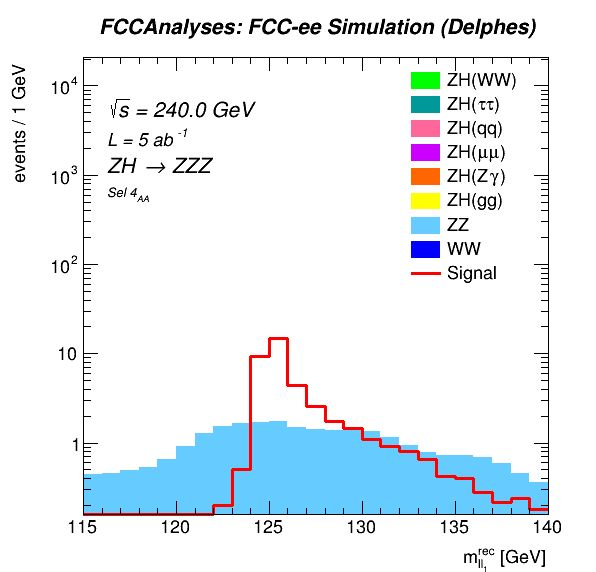
\includegraphics[width = 2.5in]{mrecll1_fit_lllljj.jpeg}}
        \subfloat[Discriminating Variable of the $Z_1(\textcolor{red}{ll})Z_2(\textcolor{NavyBlue}{jj})Z_3(\textcolor{red}{ll})$ Enhanced Signature\\($m_{jj+ll_3}$)]{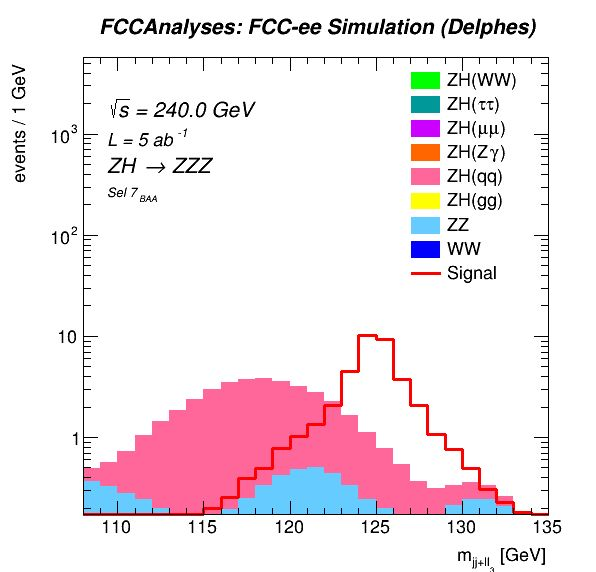
\includegraphics[width = 2.5in]{mjjll3_fit_lljjll.jpeg}}\\
        \subfloat[Discriminating Variable of the $Z_1(\textcolor{NavyBlue}{jj})Z_2(\textcolor{red}{ll})Z_3(\textcolor{red}{ll})$ Enhanced Signature\\($m_{ll_2+ll_3}$)]{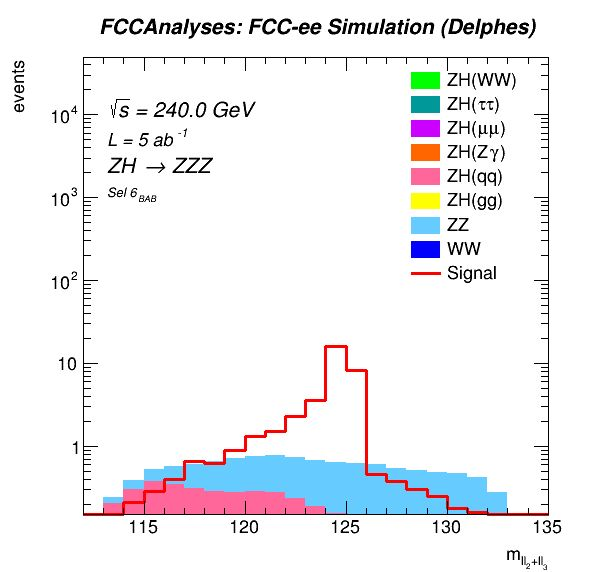
\includegraphics[width = 2.5in]{mll2ll3_fit_jjllll.jpeg}}
        \subfloat[Discriminating Variable of the $Z_1(\textcolor{Green}{\nu\nu})Z_2(\textcolor{red}{ll})Z_3(\textcolor{red}{ll})$ Enhanced Signature\\($m_{ll_2+ll_3}$)]{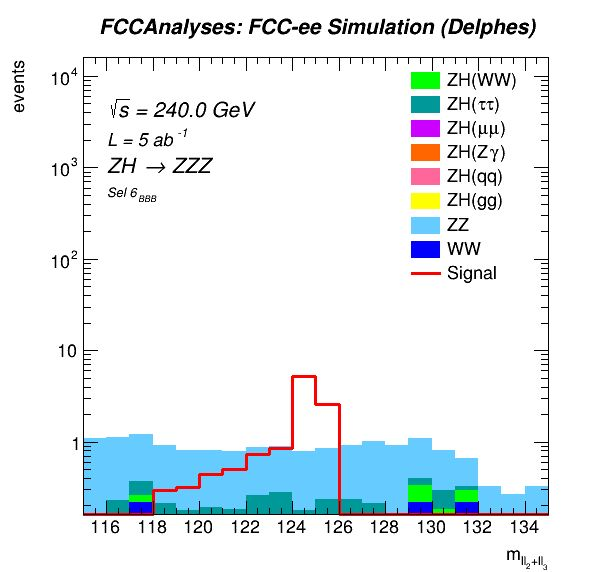
\includegraphics[width = 2.5in]{mll2ll3_fit_vvllll.jpeg}}
        \caption{Distribution of the discriminating variables used for the statistical treatment.}
        \label{DicsriminatingVariables}
    \end{figure}

    \noindent
    Before performing the fit, 10 \% systematic uncertainties are added to the most abundant backgrounds in the final distributions: $ZZ$ for $\textcolor{red}{llll}\textcolor{NavyBlue}{jj}$ and $\textcolor{Green}{\nu\nu}\textcolor{red}{llll}$; $ZZ$ and $ZH(qq)$ for $\textcolor{red}{ll}\textcolor{NavyBlue}{jj}\textcolor{red}{ll}$ and $\textcolor{red}{ll}\textcolor{Green}{\nu\nu}\textcolor{red}{ll}$. These systematic uncertainties are considered independent between the channels. We obtain the following fit results when considering each channel separately:
    \begin{center}
        $\mu_{\textcolor{red}{llll}\textcolor{NavyBlue}{jj}}=1\substack{+0.193\\-0.176}$\\
        \vspace{0.2cm}
        $\mu_{\textcolor{red}{ll}\textcolor{NavyBlue}{jj}\textcolor{red}{ll}}=1\substack{+0.193\\-0.174}$\\
        \vspace{0.2cm}
        $\mu_{\textcolor{NavyBlue}{jj}\textcolor{red}{llll}}=1\substack{+0.187\\-0.168}$\\
        \vspace{0.2cm}
        $\mu_{\textcolor{Green}{\nu\nu}\textcolor{red}{llll}}=1\substack{+0.394\\-0.329}$
    \end{center}    

    \noindent
    \\To have the lowest possible uncertainty, the four channels are considered all together, each one with its chosen distribution. After performing the fit on the four channels listed in Table \ref{FitChannels}, we obtain the following combined result:$$\boxed{\mu=1\substack{+0.104\\-0.098}}$$
    \underline{Note}: when applying the fit on many channels simultaneously, one must be careful about the orthogonality of the considered channels. Otherwise, same events may be counted twice, or more, if they are encountered in more than one channel. In our analysis, all the considered channels are orthogonal thanks to the selections. The orthogonality of the channels is showed in Figure \ref{Orthogonality}.\\
    \begin{figure}[h!]
        \centering
        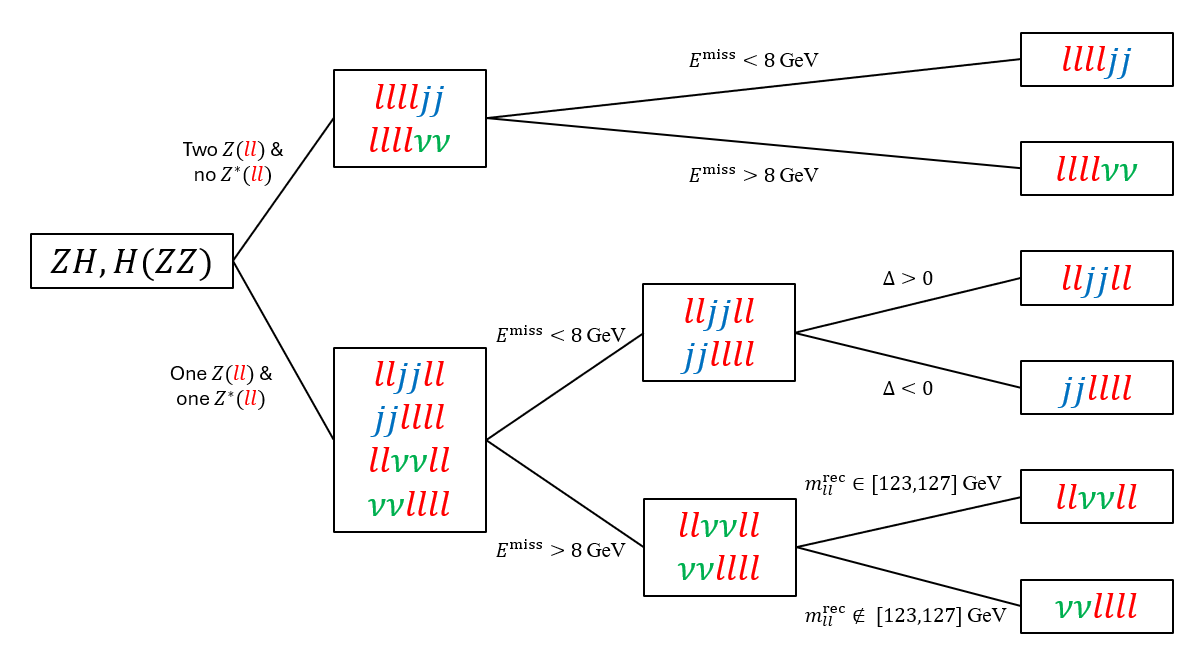
\includegraphics[scale=0.5]{Orthogonality.png}
        \caption[Diagram showing the orthogonality of the considered channels through the selections.]
        {Diagram showing the orthogonality of the considered channels through the selections.\\$\Delta$ is defined as: $\Delta=|125\;\mbox{GeV}-m^{\mbox{rec}}_{jj}|-|125\;\mbox{GeV}-m^{\mbox{rec}}_{ll}|$}
        \label{Orthogonality}
    \end{figure}

    \noindent
    To see how much the systematic uncertainties affected the total uncertainty on the POI, $\delta^{\mbox{tot}}_\mu$, the fit is performed with the systematic uncertainties set to 0. This gives $\mu=1\pm\delta^{\mbox{stat}}_\mu$ where $\delta^{\mbox{stat}}_\mu$ is the statistical uncertainty. As shown in Table \ref{ChannelUncertainties}, the total uncertainty is dominated by the statistical uncertainty. Indeed, the contribution of the systematic uncertainties is seen in the third decimal place.
    \begin{table}[h!]
        \centering
        \begin{tabular}{|c|c|c|}
            \hline
            Channel & $\delta^{\mbox{stat}}_\mu$ & $\delta^{\mbox{tot}}_\mu$ \\
            \hline
            $Z_1(\textcolor{red}{ll})Z_2(\textcolor{red}{ll})Z_3(\textcolor{NavyBlue}{jj})$ & \thead{$+0.191$\\$-0.173$} & \thead{$+0.193$\\$-0.176$} \\
            $Z_1(\textcolor{red}{ll})Z_2(\textcolor{NavyBlue}{jj})Z_3(\textcolor{red}{ll})$ & \thead{$+0.191$\\$-0.173$} & \thead{$+0.193$\\$-0.174$} \\
            $Z_1(\textcolor{NavyBlue}{jj})Z_2(\textcolor{red}{ll})Z_3(\textcolor{red}{ll})$ & \thead{$+0.186$\\$-0.168$} & \thead{$+0.187$\\$-0.168$} \\
            $Z_1(\textcolor{Green}{\nu\nu})Z_2(\textcolor{red}{ll})Z_3(\textcolor{red}{ll})$ & \thead{$+0.393$\\$-0.327$} & \thead{$+0.394$\\$-0.329$} \\
            Combination & \thead{$+0.103$\\$-0.097$} & \thead{$+0.104$\\$-0.098$} \\
            \hline
        \end{tabular}
        \caption{Statistical and total uncertainty on the POI for the channels considered for the statistical treatment.}
        \label{ChannelUncertainties}
    \end{table}
    
	\subsection{Encountered Difficulties During the Pseudo-Data Analysis}
    The first encountered difficulty during the data analysis was regarding the $Z_1(\textcolor{red}{ll})Z_2(\textcolor{red}{ll})Z_3(\textcolor{Green}{\nu\nu})$ channel. Indeed, as it can be seen in Table \ref{Cutflowllllvv}, this channel suffers from a lot of background coming from $ZH(\tau\tau)$ in addition to $ZZ$ background. One would be tempted to look at the recoil mass of $Z_1$ ($\boldsymbol{m^{\mbox{rec}}_{ll_1}}$) as a discriminating variable for this channel, however, as shown in Figure \ref{mrecll1_llllvv}, this variable does not separate the signal from $ZH(\tau\tau)$.\\\\
    Another encountered difficulty concerned the missing four-vector whose invariant mass was set to 0 GeV by default\footnote{In the simulated data, the missing four-vector is defined as $(p^{\mbox{miss}}_x,p^{\mbox{miss}}_y,p^{\mbox{miss}}_z,m^{\mbox{miss}})=(p^{\mbox{miss}}_x,p^{\mbox{miss}}_y,p^{\mbox{miss}}_z,0)$}. For the $Z_1(\textcolor{red}{ll})Z_2(\textcolor{Green}{\nu\nu})Z_3(\textcolor{red}{ll})$ channel, one would like to use as a discriminating variable $\boldsymbol{m_{\nu\nu+ll_3}}$, which is the invariant mass of the four-vector obtained by summing the missing four-vector and the $Z_3$ four-vector. Indeed, $\boldsymbol{m_{\nu\nu+ll_3}}$ should show a resonance at 125 GeV for the signal as the neutrinos and the leptonic off-shell $Z$ boson come from the Higgs boson. However, this is not verified for the given definition of the missing four-vector. To remedy this, we reset the invariant mass of the missing four-vector at 91 GeV\footnote{The missing four-vector was redefined as $(p^{\mbox{miss}}_x,p^{\mbox{miss}}_y,p^{\mbox{miss}}_z,m^{\mbox{miss}})=(p^{\mbox{miss}}_x,p^{\mbox{miss}}_y,p^{\mbox{miss}}_z,91)$} when looking at $Z_1(\textcolor{red}{ll})Z_2(\textcolor{Green}{\nu\nu})Z_3(\textcolor{red}{ll})$ as the neutrinos come from an on-shell $Z$ boson. This allow us to have the expected resonance at 125 GeV for $\boldsymbol{m_{\nu\nu+ll_3}}$ as shown in Figure \ref{mvvll3}. This distribution was still not used for the statistical treatment due to high contamination from $ZH(\tau\tau)$, $ZH(WW)$ and $ZZ$ which are yet to be reduced.
    \begin{table}[ht]
    \centering
    \begin{minipage}[h]{0.4\textwidth}
        \centering
        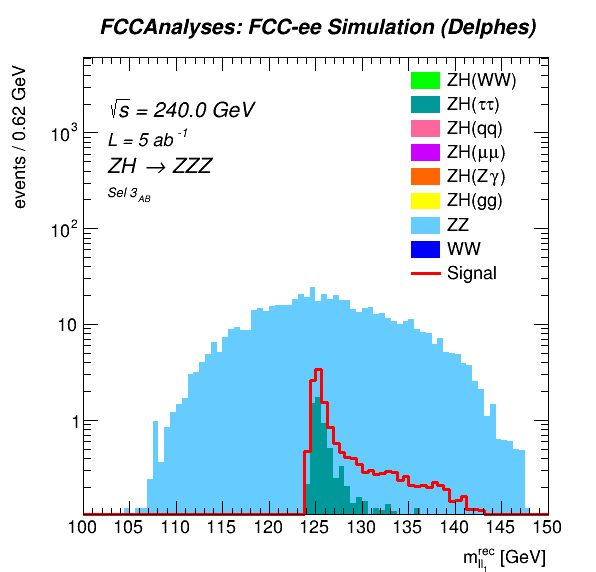
\includegraphics[scale=0.35]{mrecll1_llllvv.jpeg}
        \captionof{figure}{Distribution of the recoil mass of $Z_1$ for the $Z_1(\textcolor{red}{ll})Z_2(\textcolor{red}{ll})Z_3(\textcolor{Green}{\nu\nu})$ enhanced signature.}
        \label{mrecll1_llllvv}
    \end{minipage}
    \hspace{0.5 in}
    \begin{minipage}[h]{0.47\textwidth}
        \centering
        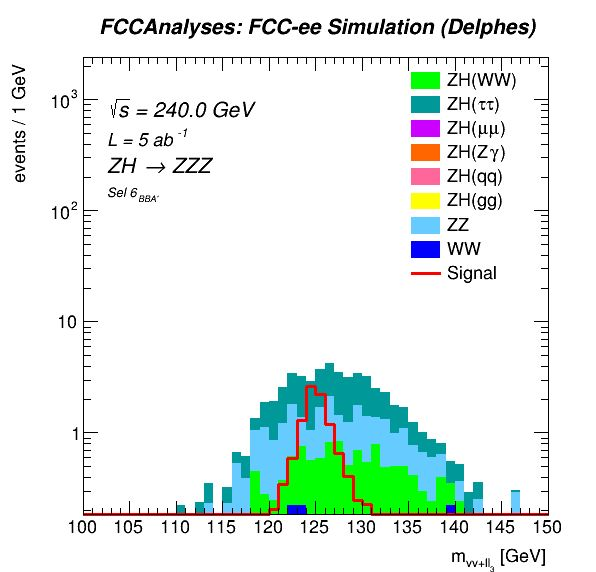
\includegraphics[scale=0.35]{mvvll3.jpeg}
        \captionof{figure}{Distribution of the mass of ($\nu\nu+Z_3$) for the $Z_1(\textcolor{red}{ll})Z_2(\textcolor{Green}{\nu\nu})Z_3(\textcolor{red}{ll})$ enhanced signature after resetting the missing mass at 91 GeV.}
        \label{mvvll3}
    \end{minipage}
    \end{table}
    
	\section{Conclusion}
    The goal of this internship was to work on a preliminary measurement of the $ZH,H\rightarrow ZZ^*$ cross section at FCC-ee in Higgs Strahlung decays with four leptons in the final state. In this regard, FCC-ee simulations at $\sqrt{s}=240$ GeV, based on the IDEA detector concept, were used.\\\\
    The $ZH,H(ZZ^*)$ decay with four leptons in the final state encounters six different combinations; two out of the three $Z$ bosons decay into a pair of leptons and the remaining $Z$ boson decay into either two jets or two neutrinos. Along the pseudo-data analysis, the six channels were considered. A series of rectangular cuts on kinematic variables was applied according to the channels' signatures in order to reduce the background events. After all the selections, four out of the six channels were used for the fit as they presented clear discriminating variables and the best signal over background ratios. The combination of the four channels gave a fit result with an uncertainty of $\sim 10\;\%$ which was dominated by statistical uncertainty. The two channels that were not used for the fit are the channels where one of the $Z$ bosons coming from the Higgs boson, $Z_2$ or $Z_3$, decays into two neutrinos. Indeed, for $Z_2\rightarrow \nu\nu$, there was a lot of contamination coming from the $ZH,H(\tau\tau)$, $ZH,H(WW)$ and $ZZ$ backgrounds and the signal was still indistinguishable after the final selection. For $Z_3\rightarrow \nu\nu$, a discriminating variable is yet to be found to distinguish the signal from the $ZH,H(\tau\tau)$ background.\\\\
    This work falls within the feasibility study of the FCC-ee project which should end in 2025. If the project is approved, it would open a huge opportunity to measure the SM predictions with high precision which could lead to finding signs of new physics if any deviations from the predictions are observed. The so-called Higgs factory puts the Higgs boson at the centre of this quest as it became a powerful tool to explore the manifestation of the SM since its discovery.\\\\
    To conclude, this internship has allowed me to confirm my decision to pursue a research career in particle physics in the future. It made me discover working in this field in a very interesting and enriching way and I have enjoyed every bit of it!
	
	%--------------------------------------
	%	REFERENCES
	%--------------------------------------
	
	\newpage
	\addcontentsline{toc}{section}{\protect\numberline{}References}
	\printbibliography

    %--------------------------------------
	%	APPENDIX
	%--------------------------------------

    \newpage
    \begin{appendices}
    \section{Variables Used for Rectangular Cuts} \label{CutflowVariables}
    
    \begin{figure}[h!]
        \centering
        \subfloat[Mass of $Z_1$]{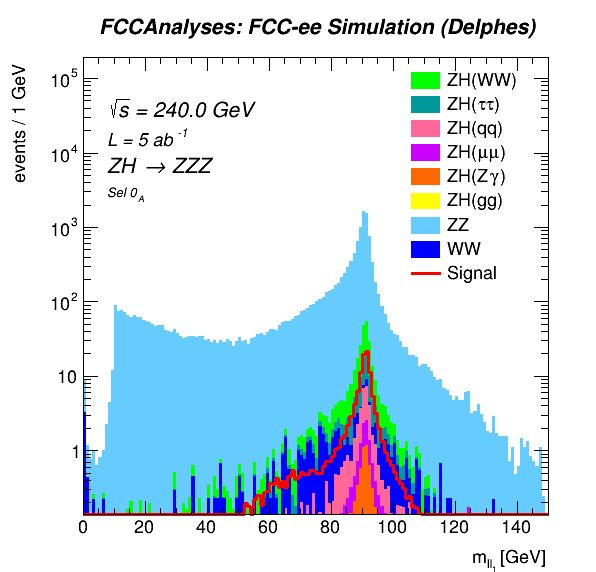
\includegraphics[width = 2.25in]{mll1_1.jpeg}} 
        \subfloat[Mass of $Z_2$]{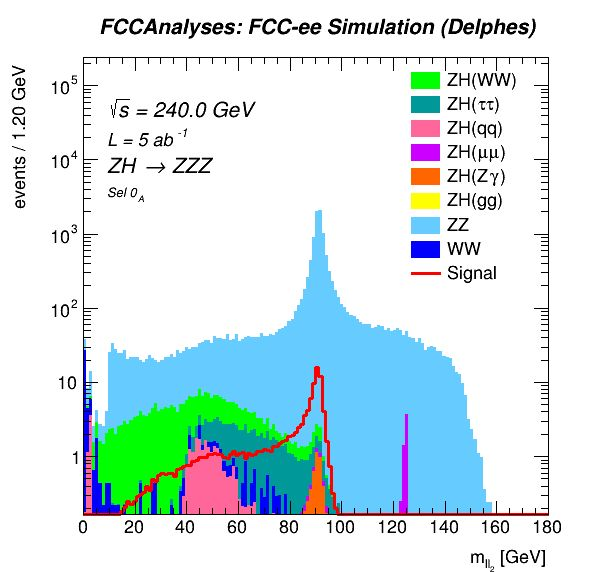
\includegraphics[width = 2.25in]{mll2_1.jpeg}}
        \subfloat[Missing Energy]{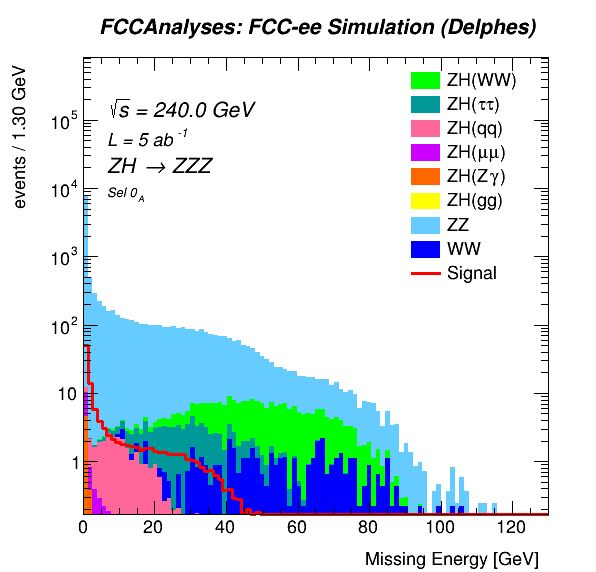
\includegraphics[width = 2.25in]{Emiss_1.jpeg}}\\
        \subfloat[Energy of the Highest-Energy Photon]{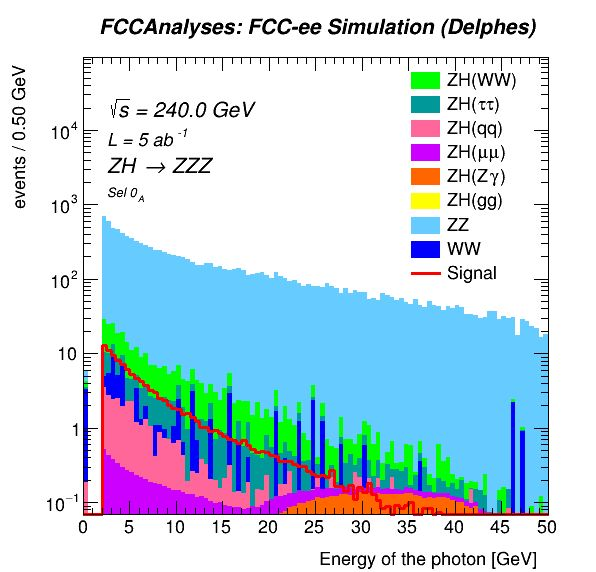
\includegraphics[width = 2.25in]{Egamma_1.jpeg}}
        \subfloat[Recoil Mass of $(Z_2+\gamma)$]{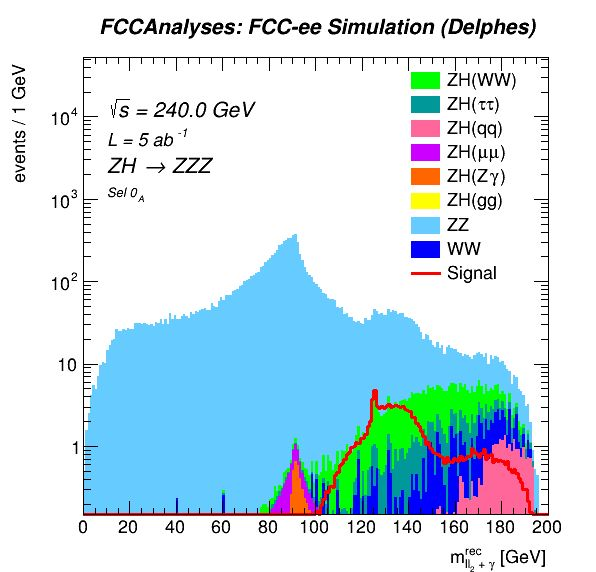
\includegraphics[width = 2.25in]{mrecll2gamma_1.jpeg}}\\
        %\subfloat[Recoil Mass of $Z_1$]{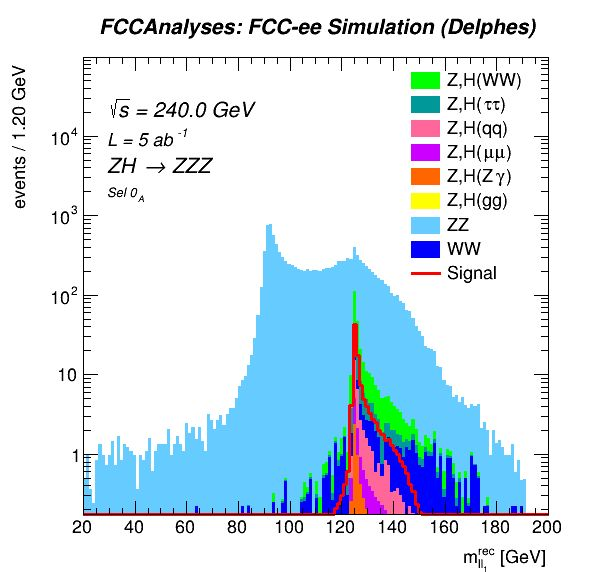
\includegraphics[width = 2.25in]{mrecll1_1.jpeg}}
        \subfloat[Recoil Mass of $Z_2$]{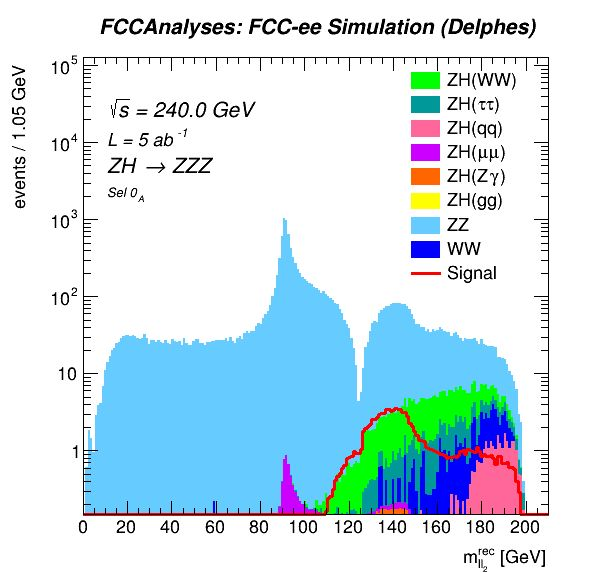
\includegraphics[width = 2.25in]{mrecll2_1.jpeg}}
        \caption[Distribution of the variables cut on in the case of $Z_1(\textcolor{red}{ll})Z_2(\textcolor{red}{ll})Z_3(xx)$.]%
        {Distribution of the variables cut on in the case of $Z_1(\textcolor{red}{ll})Z_2(\textcolor{red}{ll})Z_3(xx)$.\\These are distributions after the preselection which requires two on-shell leptonic $Z$ bosons (Sel $0_A$).}
        \label{Variables_1}
    \end{figure}

    \newpage
    \begin{figure}[h!]
        \centering
        \subfloat[Mass of the On-Shell Z]{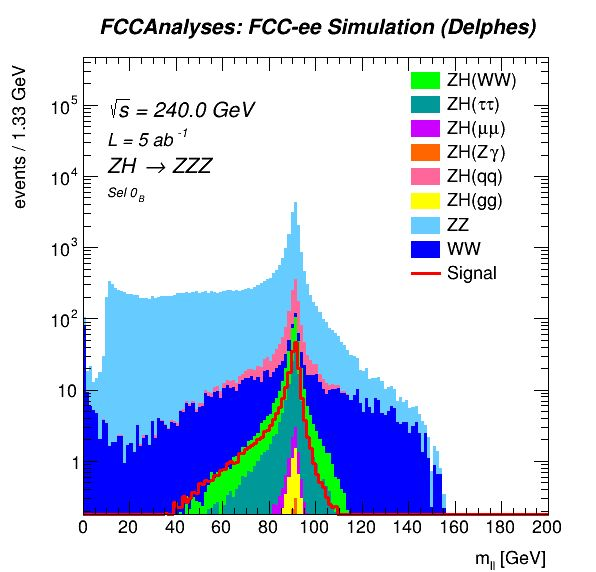
\includegraphics[width = 2.25in]{mll_2.jpeg}} 
        \subfloat[Mass of $Z_3$]{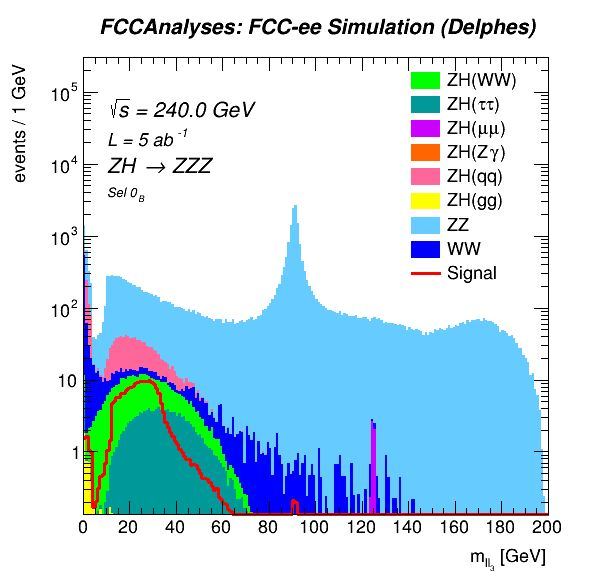
\includegraphics[width = 2.25in]{mll3_2.jpeg}}
        \subfloat[Missing Energy]{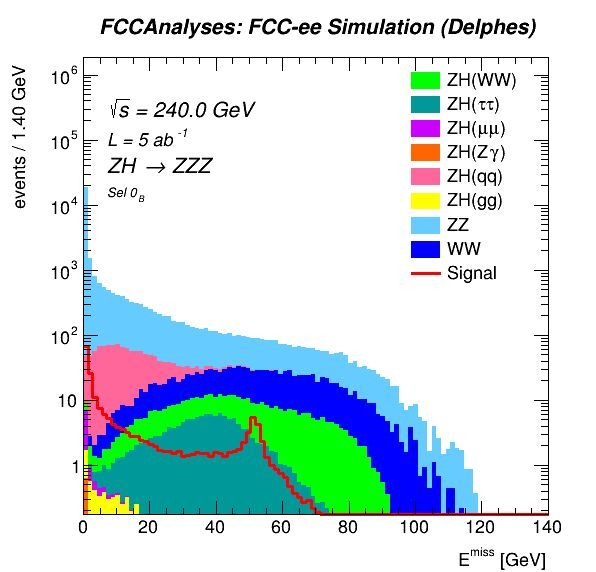
\includegraphics[width = 2.25in]{Emiss_2.jpeg}}\\
        \subfloat[Mass of the Dijet]{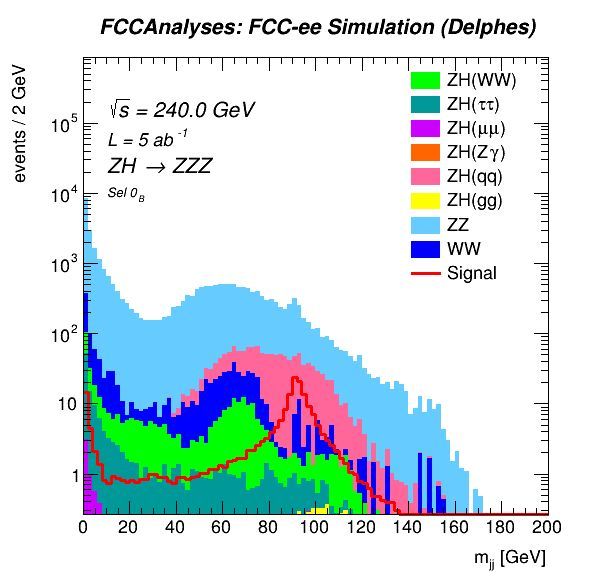
\includegraphics[width = 2.25in]{mjj_2.jpeg}}
        \subfloat[Recoil Mass of $Z_3$]{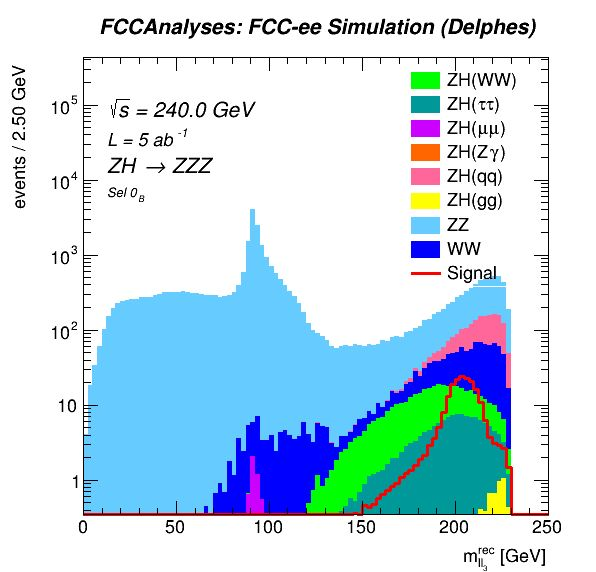
\includegraphics[width = 2.25in]{mrecll3_2.jpeg}}
        \subfloat[Recoil Mass of $(jj+Z_3)$]{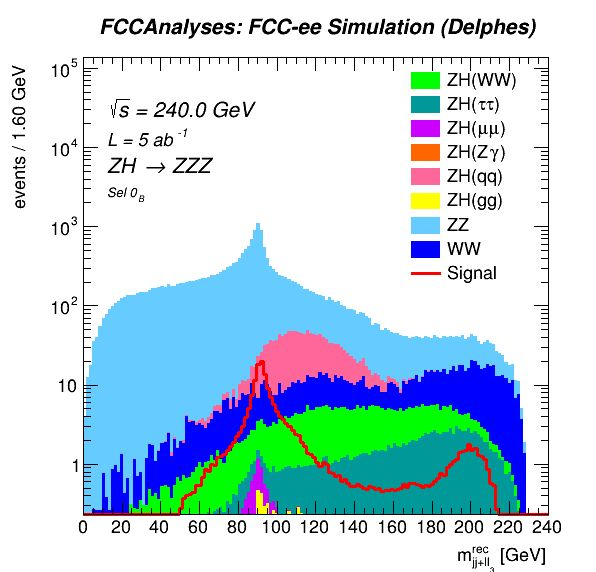
\includegraphics[width = 2.25in]{mrecll3jj_2.jpeg}}\\
        \subfloat[Recoil Mass of the On-Shell Z]{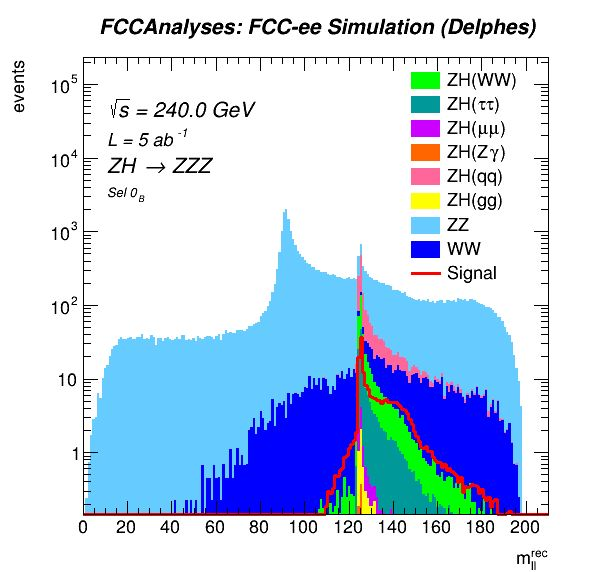
\includegraphics[width = 2.25in]{mrecll_2.jpeg}}
        \subfloat[Visible Mass
        ]{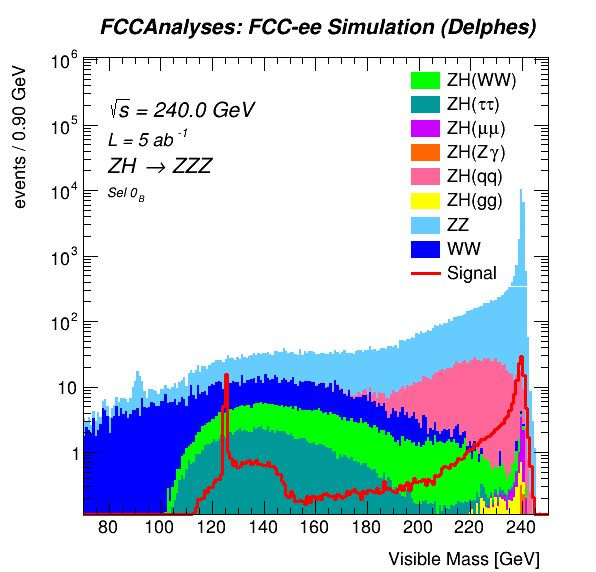
\includegraphics[width = 2.25in]{mvis_2.jpeg}}
        \caption[Distribution of the variables cut on in the case of $Z_1(\textcolor{red}{ll})Z_2(xx)Z_3(\textcolor{red}{ll})$ and $Z_1(xx)Z_2(\textcolor{red}{ll})Z_3(\textcolor{red}{ll})$.]%
        {Distribution of the variables cut on in the case of $Z_1(\textcolor{red}{ll})Z_2(xx)Z_3(\textcolor{red}{ll})$ and $Z_1(xx)Z_2(\textcolor{red}{ll})Z_3(\textcolor{red}{ll})$.\\These are distributions after the preselection which requires one on-shell and one off-shell leptonic $Z$ bosons (Sel $0_B$)
        .}
        \label{Variables_2}
    \end{figure}

    \newpage
    \section{Discriminating Variables Before the Smoothing} \label{NoSmoothing}
    \begin{figure}[h!]
        \centering
        \subfloat[Discriminating Variable of the $Z_1(\textcolor{red}{ll})Z_2(\textcolor{red}{ll})Z_3(\textcolor{NavyBlue}{jj})$ Enhanced Signature\\($m^{\mbox{rec}}_{ll_1}$)]{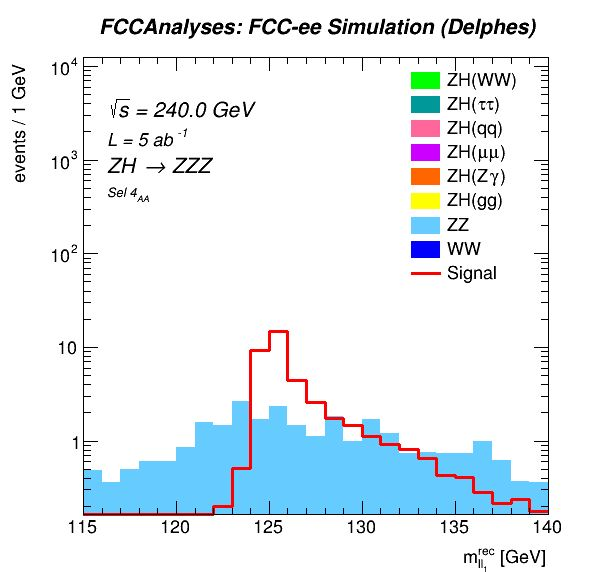
\includegraphics[width = 2.5in]{mrecll1_fit_lllljj_NS.jpeg}}
        \subfloat[Discriminating Variable of the $Z_1(\textcolor{red}{ll})Z_2(\textcolor{NavyBlue}{jj})Z_3(\textcolor{red}{ll})$ Enhanced Signature\\($m_{jj+ll_3}$)]{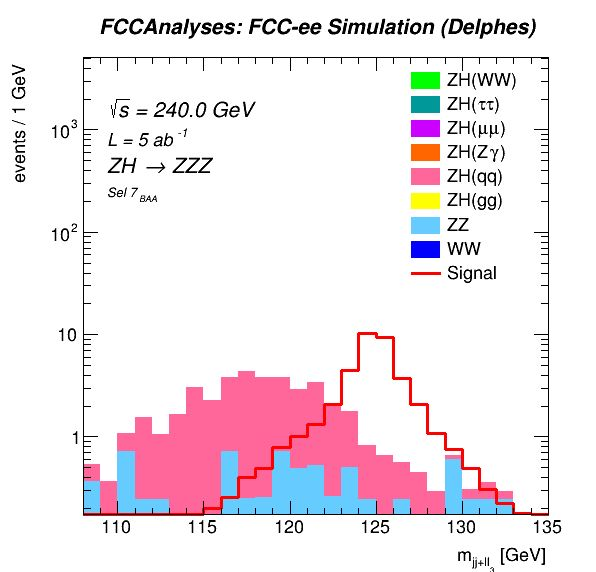
\includegraphics[width = 2.5in]{mjjll3_fit_lljjll_NS.jpeg}}\\
        \subfloat[Discriminating Variable of the $Z_1(\textcolor{NavyBlue}{jj})Z_2(\textcolor{red}{ll})Z_3(\textcolor{red}{ll})$ Enhanced Signature\\($m_{ll_2+ll_3}$)]{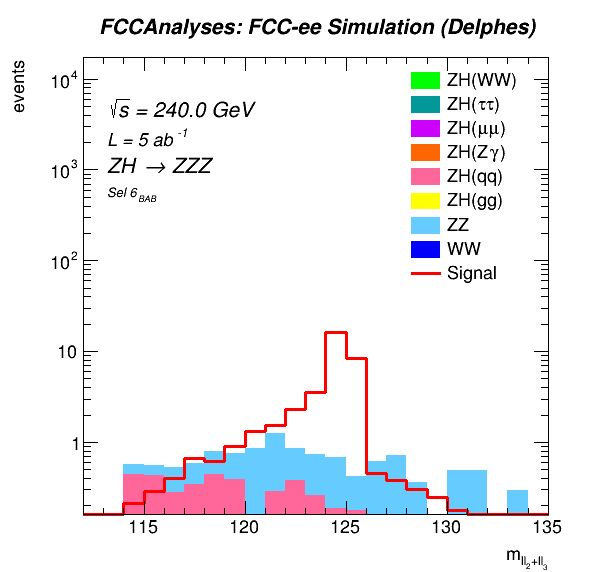
\includegraphics[width = 2.5in]{mll2ll3_fit_jjllll_NS.jpeg}}
        \subfloat[Discriminating Variable of the $Z_1(\textcolor{Green}{\nu\nu})Z_2(\textcolor{red}{ll})Z_3(\textcolor{red}{ll})$ Enhanced Signature\\($m_{ll_2+ll_3}$)]{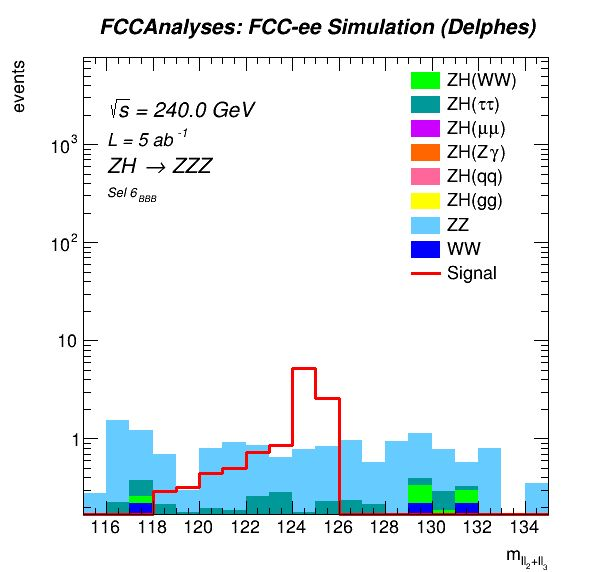
\includegraphics[width = 2.5in]{mll2ll3_fit_vvllll_NS.jpeg}}
        \caption{Distribution of the discriminating variables before the smoothing.}
        \label{DicsriminatingVariablesNS}
    \end{figure}

    \newpage
    \section{Summary of Studied Channels}
    \begin{table}[h!]
        \centering
        %\begin{adjustbox}{width=1\textwidth}
        \begin{tabular}{|c|c|c|}
            \hline
            Channel & $S/B$ & $S/\sqrt{B}$ \\
            \hline
            $Z_1(\textcolor{red}{ll})Z_2(\textcolor{red}{ll})Z_3(\textcolor{NavyBlue}{jj})$ & $\sim 1.5$ & $\sim 7.9$ \\
            $Z_1(\textcolor{red}{ll})Z_2(\textcolor{NavyBlue}{jj})Z_3(\textcolor{red}{ll})$ & $\sim 0.95$ & $\sim 6.2$ \\
            $Z_1(\textcolor{NavyBlue}{jj})Z_2(\textcolor{red}{ll})Z_3(\textcolor{red}{ll})$ & $\sim 3.1$ & $\sim 10.9$ \\
            $Z_1(\textcolor{Green}{\nu\nu})Z_2(\textcolor{red}{ll})Z_3(\textcolor{red}{ll})$ & $\sim 0.75$ & $\sim 2.9$ \\
            \hline
            $Z_1(\textcolor{red}{ll})Z_2(\textcolor{Green}{\nu\nu})Z_3(\textcolor{NavyBlue}{jj})$ & $\sim 1.06$ & $\sim 11.7$ \\
            $Z_1(\textcolor{red}{ll})Z_2(\textcolor{NavyBlue}{jj})Z_3(\textcolor{Green}{\nu\nu})$ & $\sim 0.30$ & $\sim 4.57$ \\
            $Z_1(\textcolor{Green}{\nu\nu})Z_2(\textcolor{red}{ll})Z_3(\textcolor{NavyBlue}{jj})$ & $\sim 0.55$ & $\sim 8.90$ \\
            $Z_1(\textcolor{red}{ll})Z_2(\textcolor{NavyBlue}{jj})Z_3(\textcolor{NavyBlue}{jj})$ & $\sim 0.039$ & $\sim 4.58$ \\
            \hline
        \end{tabular}
        %\end{adjustbox}
        \caption[Signal over background ratios for the channels studied in this report and the channels studied by Ines Combes.]
        {Signal over background ratios for the channels studied in this report (four first) and the channels studied by Ines Combes \cite{InesCombes2023} (four last).\\$S$ is the number of signal events and $B$ is the total number of background events.}
        \label{SummaryTable}
    \end{table}
	
    \end{appendices}
 
\end{document}